%%%%%%%%%%%%%%%%%%%%%%%%%%%%%%%%%%%%%%%%%%%%%%%%%%%%%%%%%%%%%%%%%%%%%%%%%%%%%%%%
%                         FORMATO DE TESIS FI UNAM                             %
%%%%%%%%%%%%%%%%%%%%%%%%%%%%%%%%%%%%%%%%%%%%%%%%%%%%%%%%%%%%%%%%%%%%%%%%%%%%%%%%
% based on Harish Bhanderi's PhD/MPhil template, then Uni Cambridge
% http://www-h.eng.cam.ac.uk/help/tpl/textprocessing/ThesisStyle/
% corrected and extended in 2007 by Jakob Suckale, then MPI-iCBG PhD programme
% and made available through OpenWetWare.org - the free biology wiki

%                     Under GNU License v3

% ADAPTADO PARA FI-UNAM:  @Tepexic

\documentclass[12pt]{Latex/Classes/PhDthesisPSnPDF}
%         PUEDEN INCLUIR EN ESTE ESPACIO LOS PAQUETES EXTRA, O BIEN, EN EL ARCHIVO "PhDthesisPSnPDF.cls" EN "./Latex/Classes/"

\usepackage[autocite=superscript, hyperref=true, sorting=nty, backref=true, backend=biber, style=apa, citestyle=authoryear]{biblatex}
\DeclareLanguageMapping{spanish}{spanish-apa}
\addbibresource{Bibliografia/referencias.bib}
\renewcommand*{\nameyeardelim}{\addcomma\space}

\DefineBibliographyStrings{spanish}{%
  backrefpage = {page},% originally "cited on page"
  backrefpages = {pages},% originally "cited on pages"
  andothers = {et\addabbrvspace al\adddot},
  and = {\&}
}

\DeclareCiteCommand{\citeauthor}
  {\boolfalse{citetracker}%
   \boolfalse{pagetracker}%
   \usebibmacro{prenote}}
  {\ifciteindex
     {\indexnames{labelname}}
     {}%
   \printtext[bibhyperref]{\printnames{labelname}}}
  {\multicitedelim}
  {\usebibmacro{postnote}}

\DeclareCiteCommand{\citeyear}
    {}
    {\bibhyperref{\printfield{year}}}
    {\multicitedelim}
    {}

\DeclareCiteCommand{\citeyearpar}
    {}
    {\mkbibparens{\bibhyperref{\printfield{year}}}}
    {\multicitedelim}
    {}

\usepackage[ pdftex, plainpages = false, pdfpagelabels, pdfpagelayout = OneColumn, bookmarks, bookmarksopen = true, bookmarksnumbered = true, breaklinks = true, linktocpage, colorlinks = true,linkcolor = black, urlcolor  = black, citecolor = black, anchorcolor = black, hyperindex = true, hyperfigures]{hyperref}

\usepackage{enumerate} % enumerados
\usepackage[chapter,Algorithm,ruled]{algorithm}
\usepackage{verbatim}
%\usepackage{algorithmic}
\usepackage{amsfonts}
\usepackage{algpseudocode}
\usepackage{setspace}
\usepackage{url}
\usepackage{float}
\usepackage{booktabs}



% http://ftp.isu.edu.tw/pub/Unix/CTAN/macros/latex/contrib/caption/caption.pdf
\usepackage[font=small]{caption}


\usepackage{graphicx}
\usepackage{subfigure}

\usepackage{times}

\usepackage[left=3cm, right=3cm,top=2.5cm,bottom=2.5cm,footskip=1.25cm]{geometry}

\usepackage{algorithmicx}


\usepackage{csquotes}

\usepackage{multirow}

\usepackage{tabularx}

\usepackage{ragged2e}
\usepackage{anyfontsize}
\usepackage{minibox}
\usepackage{setspace}
\newcommand{\tabitem}{~~\llap{\textbullet}~~}
\newcommand\pro{\item[$+$]}
\newcommand\con{\item[$-$]}

\usepackage[final]{pdfpages}

%%%%%%%%%%%%%%%%%%%%%%%%%%%%%%%%%%%%%%%%%%%%%%%%%%%%%
%                   PORTADA                         %
%%%%%%%%%%%%%%%%%%%%%%%%%%%%%%%%%%%%%%%%%%%%%%%%%%%%%
\begin{document}

\begin{titlepage}

    \begin{center}
        
        \vspace*{-0.15cm}
    
        \minibox[c]{\fontsize{18}{30}\selectfont \LARGE{SEP} \hfill \LARGE{TNM}  \\[0.25cm]
        \fontsize{20}{30}\selectfont INSTITUTO TECNOLÓGICO DE CULIACÁN}
        
        \vspace{0.25cm}
        
        \begin{figure}[H]
            \centering
            
\includegraphics[scale=0.25]{Portada/logotec.png}
        \end{figure}
        
        \vspace{0.3cm}
        \large{ESTIMACIÓN DE LA VELOCIDAD VEHICULAR A PARTIR DE SECUENCIAS DE VIDEO MEDIANTE TÉCNICAS DE VISIÓN ARTIFICIAL Y APRENDIZAJE MÁQUINA.}
        
        \vspace{0.5cm}
        
        \large{TESIS}
        
        \vspace{-0.2cm}
        
        {\fontsize{11}{30}\selectfont \justify{PRESENTADA ANTE EL DEPARTAMENTO ACADÉMICO DE ESTUDIOS DE POSGRADO DEL INSTITUTO TECNOLÓGICO DE CULIACÁN EN CUMPLIMIENTO PARCIAL DE LOS} REQUISITOS PARA OBTENER EL GRADO DE}
        
        \vspace{0.5cm}
        {\fontsize{14}{30}\selectfont MAESTRO EN CIENCIAS DE LA COMPUTACIÓN}
        
        
        \vspace{0.5cm}
        
        {\fontsize{14}{30}\selectfont POR:}
        
        \vspace{0.5cm}
        {\fontsize{11}{30}\selectfont ING. RAFAEL IMPERIAL ROJO}
        
        
        {\fontsize{14}{30}\selectfont INGENIERO EN SISTEMAS COMPUTACIONALES }
        
        
        \vspace{0.5cm}
        {\fontsize{14}{30}\selectfont DIRECTOR DE TESIS:}
        
        {\fontsize{11}{30}\selectfont DR. HÉCTOR RODRÍGUEZ RANGEL}
        
        \vspace{2.5cm}
        {\fontsize{14}{30}\selectfont CULIACÁN, SINALOA} \hfill {\fontsize{14}{30}\selectfont DD de MM del 2021}
        
        
    \end{center}

\end{titlepage}

%\maketitle									% Se redefinió este comando en el archivo de la clase para generar automáticamente la portada a partir de los datos

%%%%%%%%%%%%%%%%%%%%%%%%%%%%%%%%%%%%%%%%%%%%%%%%%%%%%
%                  PRÓLOGO                          %
%%%%%%%%%%%%%%%%%%%%%%%%%%%%%%%%%%%%%%%%%%%%%%%%%%%%%
\frontmatter

% \newpage
% \thispagestyle{empty}
% \mbox{}

% \newpage
% \thispagestyle{empty}
% \mbox{}



% \newpage
% \thispagestyle{empty}
% \mbox{}

% \newpage
% \thispagestyle{empty}
% \mbox{}
\pagestyle{plain}
\vspace{0.5cm}

\includepdf[]{Prologo/pdf/Autorizacion}

\includepdf[]{Prologo/pdf/HojaFirmas}

\noindent {\fontsize{24}{30}\selectfont \textbf{Dedicatoria}}

\begin{spacing}{1.5}

Dedico este trabajo a mis padres Rosa Haydee Rojo Acosta y Rafael Imperial Sánchez quienes me han apoyado a lo largo de mi vida. Gracias a esto he podido plantearme metas a largo plazo, siendo un logro más alcanzar el nivel de maestría en mi carrera profesional, este logro también es de ellos. Se han esforzado en apoyarme, aconsejarme y dar lo mejor de ellos para mi crecimiento personal.

\end{spacing}


\newpage

\noindent {\fontsize{24}{30}\selectfont \textbf{Agradecimientos}}

\begin{spacing}{1.8}

\noindent Agradezco a \textbf{mi familia} por su apoyo y motivación durante mis estudios.
\\
\noindent Al \textbf{Instituto Tecnológico de Culiacán} por mi formación profesional en licenciatura y maestría.
\\
\noindent Al \textbf{Consejo Nacional de Ciencia y Tecnología} por financiar mis estudios de maestría.
\\
\noindent A \textbf{mis compañeros} por su apoyo y volverse mis amigos en el poco tiempo que hemos estado conviviendo como compañeros.
\\
\noindent Al \textbf{Dr. Héctor Rodríguez Rangel} por su apoyo, su paciencia, sus aportes y compartir conmigo sus experiencias para que yo pueda alcanzar esta meta.
\\
\noindent Al \textbf{profesorado y personal de posgrado} compartir sus conocimientos, su apoyo y su gestión del departamento de Posgrado.
\\
\noindent Por último, a la \textbf{Dra. María Lucia Barrón} Estrada sin su apoyo y confianza no habría podido ingresar a esta Maestría, su labor como profesora para mí ha sido la más importante en mi carrera al enseñarme las bases de todo lo que se hoy en día, gracias a ella fue que nació en mi la pasión por la informática.

\end{spacing} 
\newpage
\noindent {\fontsize{24}{30}\selectfont \textbf{Declaración de autenticidad}}

\begin{spacing}{1.5}
    \noindent Por la presente declaro que, salvo cuando se haga referencia específica al trabajo de otras personas, el contenido de esta tesis es original y no se ha presentado total o parcialmente para su consideración para cualquier otro título o grado en esta o cualquier otra Universidad. Esta tesis es resultado de mi propio trabajo y no incluye nada que sea resultado de algún trabajo realizado en colaboración, salvo que se indique específicamente en el texto.
\end{spacing}


\begin{flushright}
Rafael Imperial Rojo. Culiacán, Sinaloa, México, 2021.
\end{flushright}
\newpage

\noindent {\fontsize{24}{30}\selectfont \textbf{Resumen}}

\begin{spacing}{1.5}

La movilidad urbana se incrementó con el uso de automóviles, lo que originó también un aumento de accidentes de tránsito. Para estudiar este fenómeno se requiere de estudios de tránsito mediante equipo especial. Con los avances tecnológicos, la inteligencia artificial y el uso de videos es posible realizarlos sin modificar en gran medida la infraestructura urbana. Para el diseño de soluciones basadas en inteligencia artificial es necesario generar bases de datos públicas que proporcionen videos confiables para la calibración y desarrollo de soluciones que permitan realizar estudios de tránsito de manera automatizada. En este trabajo se presenta un sistema para generar un conjunto de datos a partir de videos grabados en un punto de observación de una vía carretera, obteniendo un total de 532 datos para analizar, los cuales fueron separados por el carril en el que fue detectado el vehículo. Este conjunto de datos fue utilizado para realizar experimentos con métodos estadísticos de correlación. La implementación de estos modelos de aprendizaje máquina se realizó mediante el uso bibliotecas como Scikit-Learn y Tensor Flow. Los mejores resultados arrojaron un Error Absoluto Medio (MAE) de 1.872 K/H para el carril central y 2.128 K/H para el último carril, aceptable comparados con el radar de velocidad Bushnell el cual tiene una precisión de 1.609 K/H. Debido a la falta de datos no fue posible realizar pruebas en el primer carril.  


%7.74 K/H y 5.86 K/H para el carril central y el último carril respectivamente utilizando métodos estadísticos, 1.246 K/H y 0.738 K/H para el carril central y el último carril utilizando la biblioteca Scikit y con 1.872 K/H y 2.128 K/H para el carril central y el último carril utilizando el modelo creado con Tensor Flow.


\end{spacing}
\newpage
\noindent {\fontsize{24}{30}\selectfont \textbf{Palabras clave}}

\begin{spacing}{1.5}

\begin{itemize}

    \item Lorem
    
\end{itemize}

\end{spacing}
\newpage


%%%%%%%%%%%%%%%%%%%%%%%%%%%%%%%%%%%%%%%%%%%%%%%%%%%%%
%                   ÍNDICES                         %
%%%%%%%%%%%%%%%%%%%%%%%%%%%%%%%%%%%%%%%%%%%%%%%%%%%%%
%Esta sección genera el índice
\setcounter{secnumdepth}{3} % organisational level that receives a numbers
\setcounter{tocdepth}{3}    % print table of contents for level 3
\tableofcontents            % Genera el índice
%: ----------------------- list of figures/tables ------------------------
\listoffigures              % Genera el ínidce de figuras, comentar línea si no se usa
\listoftables               % Genera índice de tablas, comentar línea si no se usa


%%%%%%%%%%%%%%%%%%%%%%%%%%%%%%%%%%%%%s%%%%%%%%%%%%%%%%
%                   CONTENIDO                       %
%%%%%%%%%%%%%%%%%%%%%%%%%%%%%%%%%%%%%%%%%%%%%%%%%%%%%
% the main text starts here with the introduction, 1st chapter,...
\mainmatter
%\def\baselinestretch{1.5}                   % Interlineado de 1.5
\spacing{1.5}
\chapter{Introducción}

El aumento del uso de vehículos motorizados se debe al incremento de la población centrándose en las zonas urbanas y la necesidad de movilidad en la vida cotidiana. Como consecuencia se tiene un aumento de tráfico vehicular, lo cual conlleva a un mayor número de accidentes vehiculares y gases de efecto invernadero, afectando la salud de la población en general. El uso de automóviles es esencial en nuestra vida cotidiana. Según la organización \textit{Association for Safe International Road Travel (ASIRT)}, cada año mueren más de 1.3 millones de personas en accidentes de tráfico. Además,  entre 20 y 50 millones de personas resultan heridas o incapacitadas (\cite{zaki2020Traffic}).

En caso de accidente, la mayor responsabilidad recae en el conductor del automóvil (\cite{velazquez2017Siniestralidad}). Entre los principales factores que provocan los accidentes de tránsito se encuentran el exceso de velocidad, la conducción distraída, obstáculos en carretera, mala señalización, estado de la infraestructura vial, e iluminación. Según datos del Instituto Nacional de Estadística e Información Geográfica (INEGI, 2011), entre 1997 y 2009, los accidentes en la región aumentaron un 72.7\% en zonas urbanas y rurales (\cite{carro2019Conductas}).

Un elemento importante al revisar la causa de accidentes viales es el exceso de velocidad, por este motivo los estudios de tránsito vehicular se enfocan en revisar las causas de este elemento. Estos estudios requieren de un sistema monitoreo de velocidad eficaz. Además, se requiere de sistemas de control que asistan al conductor al transitar por las calles, conocidos como \textit{ADAS (Advanced Driver Assistance Systems)} (\cite{carro2019Conductas}).

Actualmente para un estudio de tránsito se necesita de equipo especializado para proporcionar las características que se desea analizar, uno de estos dispositivos son los radares de velocidad los cuales utilizan ondas de radio para calcular el tiempo que le toma a la onda viajar hasta el vehículo y de vuelta al radar para determinar la velocidad con la que viaja el vehículo. A su vez estos dispositivos son utilizados en puntos estratégicos de la ciudad para monitorear las velocidades vehiculares, tomar una captura del vehículo y realizar una multa por exceso de velocidad.

Ahora bien, para un estudio de tránsito se requiere equipos especializados como los radares de velocidad no es tan viable por su elevado costo. Sin embargo, actualmente las ciudades cuentan con un sistema de videovigilancia. En donde es posible usar este equipo existente en la ciudad para determinar varias características del flujo vehicular como el flujo vehicular, la velocidad, accidentes, entre otros.

La estimación del tráfico puede proporcionarse a los usuarios y a las patrullas de policía para ayudar en la planificación de las salidas y evitar aglomeramiento de vehículos mediante paneles carreteros o los monitores vehiculares integrados (\cite{impedovo2019Vehicular}).

La inteligencia artificial está revolucionando la sociedad moderna. Los investigadores y desarrolladores tanto de la industria automotriz como de seguridad vial están desarrollando activamente enfoques de conducción autónoma y monitoreo basados en el aprendizaje profundo. Para esto es necesario contar con una red neuronal capaz de detectar vehículos capturados mediante vídeo con la finalidad de determinar su velocidad, clasificarlos, detectar accidentes, por mencionar algunas tareas.

\citeauthor{rao2018Deep} describen las posibilidades y desafíos de integrar el aprendizaje profundo en vehículos autónomos en donde se estudia la creación de base de datos para el entrenamiento de dichas redes neuronales. En este trabajo se presenta un proceso y un sistema para la creación de un conjunto de datos el cual es utilizado para  determinar la velocidad de vehículos con ayuda de inteligencia artificial.



\section{Definición del problema}

Actualmente hay un incremento de la población en las grandes ciudades, entre algunas razones del crecimiento es que, estas tienden a proporcionar más trabajos. Este incremento de población ha provocado diferentes problemas entre ellos el de movilidad. En las ciudades grandes o pequeñas, los vehículos de motor son el principal medio con el cual la población es capaz de trasladarse ya sea para la recreación o para llegar a sus lugares de trabajo. El aumento de población y aumento de vehículos también son causantes de gran cantidad de emisiones de gases de efectos invernaderos, los cuales a su vez provocan problemas de salud para la población en general.

Un flujo de vehículos sin pausas prolongadas ayudan a disminuir los problemas de tráfico y la reducción de contaminación, ya que un vehículo detenido siempre continuo con el motor encendido. Mejorar el flujo vehicular es importante para disminuir las consecuencias de la gran cantidad de vehículos. Los análisis de tráfico identifican características como las horas pico, accidentes viales, la velocidad, el conteo de vehículos, entre otros. El presente trabajo está centrado en el desarrollo de una herramienta capaz de determinar la velocidad a la que viajan los vehículos a partir de secuencias de vídeo.

El enfoque tradicional para realizar estudios de tránsito está influenciado por el uso de equipo especial. Estos se pueden instalar bajo la superficie de la carretera tales como espires inductivas, sensores de campo magnético, contadores de ejes sensores capacitivos y piezoeléctricos. Por otro lado, se pueden instalar encima de la carretera, como los son los detectores de radares de microondas, detectores de radar láser, sensores de campo magnético, sensores infrarrojos pasivos y activos, sensores ultrasónicos y entre otros instrumentos, los cuales tienen un costo elevado además de necesitar una instalación especializada.

Las cámaras de videovigilancia son dispositivos instalados en puntos estratégicos de las grandes ciudades, es por esto que se busca agregarles la capacidad de medir la velocidad de los vehículos con la ayuda de inteligencia artificial, buscando aprovechar al máximo la infraestructura existente y ahorrar en los costos de nuevos dispositivos.

\section{Hipótesis}

Se puede determinar la velocidad de vehículos en movimiento en secuencias de vídeo utilizando técnicas de inteligencia artificial y visión artificial.

\section{Objetivo}

Determinar la trayectoria y velocidad de un vehículo usando secuencias de vídeo a través de técnicas de inteligencia artificial y visión artificial.

\section{Objetivos específicos}

\begin{itemize}
    \item Implementar un modelo de clasificación de vehículos mediante secuencias de vídeo usando técnicas de inteligencia artificial.
    \item Implementar algoritmos de flujo óptico para determinar la trayectoria de un vehículo.
    \item Generar un conjunto de datos que ayuden a entrenar un modelo para determinar la velocidad de vehículos.
    \item Diseñar e implementar un algoritmo para la determinación de la velocidad de vehículos mediante secuencias de vídeo.
\end{itemize}

\section{Justificación}

Con la implementación de un sistema para determinar la velocidad de vehículos en cámaras de videovigilancia, damos a los centros de monitoreo datos para analizar e identificar los puntos más importantes en los que hay que poner especial atención para evitar posibles accidentes viales que podrían costar la perdida de vidas o simplemente el retraso en los tiempos de traslados provocados por la congestión  de tráfico lo a su vez ayuda a disminuir los gases de efecto invernadero nocivos para la salud.

Además, con la integración del sistema propuesto se espera un ahorro económico, puesto que no es necesario adquirir equipo especializado para determinar la velocidad de vehículos.

\section{Estructura de la tesis}

Este trabajo está dividido en seis capítulos organizados de la siguiente manera:


\begin{itemize}
\item Capítulo 1 - Introducción: Se define el problema, la hipótesis, el objetivo, los objetivos específicos y la justificación de este trabajo.

\item Capítulo 2 - Marco teórico: Se presentan los conceptos clave inteligencia artificial y visión artificial necesarios para comprender el contenido de este trabajo.

\item Capítulo 3 - Estado del arte: Se presentan trabajos relacionados con determinar la velocidad de objetos.

\item Capítulo 4 - Metodología: Se explica el proceso para el desarrollo del sistema, así como las herramientas utilizadas y la razón de utilizar ciertas herramientas.

\item Capítulo 5 - Análisis de los resultados: Se presentan los resultados obtenidos utilizando el sistema y comparándolo con métodos convencionales como los radares de velocidad.

\item Capítulo 6 - Conclusión: Se presenta de manera resumida el proyecto, al mismo tiempo que el aporte del trabajo al área y el trabajo futuro que podría realizarse.
\end{itemize}


\chapter{Marco Teórico}

Este capítulo introduce a los conceptos más relevantes para el desarrollo del presente trabajo. Se abordan conceptos de Visión Artificial, Inteligencia Artificial, Aprendizaje Máquina, Aprendizaje Profundo, entre otros.

\section{Visión artificial}

La visión artificial intenta describir el mundo que vemos en imágenes y reconstruir sus propiedades (\cite{szeliski2010computer}), con ayuda de la visión artificial es posible darle la capacidad a una máquina para identificar, analizar y procesar imágenes del mundo real. En esta sección se explicará como, una máquina representa una imagen para después representarla en una pantalla o simplemente procesarla. Por otro lado se define el filtro Kalman el cual fue utilizado para el seguimiento de objetos.

\subsection{Representación de imágenes}

En computación una imagen se representa como una cuadrícula, donde cada recuadro es llamado píxel. Un píxel es la unidad más pequeña de la imagen y representa un color (\cite{rosebrock2017deep}). Con lo anterior se entiende, que para una imagen de 1000 x 600 se tienen, 1000 píxeles en cada fila y 600 píxeles para cada columna resultando 600,000 píxeles en total. Además, son dos las representaciones más comunes de un píxel (i.e escala de grises, color).

%\begin{itemize}
%\item Escala de grises
%\item A color
%\end{itemize}

Cuando se representa una imagen utilizando escala de grises cada píxel tiene un valor numérico en el rango de 0 a 255. Con este rango de valores es posible variar la intensidad de color presentado, siendo 0 el valor para representar el color negro y 255 el color blanco. Teniendo esto en cuenta se puede interpretar que los valores intermedios son diferentes intensidades de grises, de ahí el nombre escala de grises.

Para los píxeles a color existen diferentes espacios de colores, en este trabajo solo se hablara acerca del espacio de color RGB. Los píxeles RGB son representados usando 3 valores de intensidad para los colores rojo, verde y azul. Cada uno de estos 3 valores tiene un rango del 0 al 255 con lo cual se pueden variar los colores presentados. Al igual que la escala de grises cada uno de estos 3 valores pueden tener valores en el intervalo de 0 a 255. Al colocar los 3 valores de RGB a '0' (cero) se representa el color negro, por el contrario, para representar el color blanco los 3 valores de RGB deben ser de 255.

Ahora bien, para el caso de la representación de los videos, estos se pueden representar utilizando escala de grises o a color. Ya que los videos son una secuencia de imágenes con las cuales se genera la sensación de movimiento. Para el caso de los videos, al conjunto de imágenes que forman el video se les llama fotogramas y pueden variar en su frecuencia. A la frecuencia de imágenes contenidas en un tiempo determinado se le conoce como fotogramas por segundo. Hoy en día los fotogramas por segundo más comunes son 60, sin embargo, ya hay implementaciones con una mayor cantidad.
La resolución tanto de una imagen como de un video se establece por la cantidad de píxeles en el eje X y el eje Y. Existen diferentes resoluciones de las cuales la más común es \textit{Full HD}, en la Tabla \ref{tab:resolutions} se muestra el resto de las resoluciones más comunes.

\begin{table}[H]
    \caption{Resoluciones de video}
    \centering
    \label{tab:resolutions}
    \begin{tabular}{|c|c|c|}
    \hline
    \textbf{SIGLAS} & \textbf{NOMBRE} & \textbf{RESOLUCIÓN} \\ \hline
    \textbf{SD}     & \textit{Standard Definition} & 640 x 480 píxeles \\ \hline
    \textbf{QHD}    & \textit{Quarter of High Definition} & 960 x 540 píxeles \\ \hline
    \textbf{HD}     & \textit{High Definition} & 1.280 x 720 píxeles \\ \hline
    \textbf{FHD}    & \textit{Full HD o Full High Definition} & 1.920 x 1.080 píxeles \\ \hline
    \textbf{QHD}    & \textit{Quad High Definition} & 2.560 x 1.440 píxeles \\ \hline
    \textbf{UHD}    & \textit{Ultra High Definition} & 3.840 x 2.160 píxeles \\ \hline
    \end{tabular}
\end{table}

\subsection{Filtro Kalman}

El filtro Kalman es una solución recursiva al filtrado lineal de datos discretos (\cite{welch1995introduction}). Se encarga de estimar las variables de estado en un sistema dinámico, lo cual, en el caso del presente trabajo, implica estimar la siguiente ubicación de un vehículo identificado.

El filtro de Kalman tiene como objetivo resolver el problema general de estimar el estado $x \space \epsilon \space \mathbb{R} ^{n}$ de un proceso controlado en tiempo discreto, el cual se representa con la Ecuación \ref{eq:kalmanEstado}.

La matriz $A$  de dimensión $n\times{}n$ en la Ecuación \ref{eq:kalmanEstado} relaciona el estado en el paso de tiempo $k$ con el estado en el paso $k + 1$, en ausencia de una función de excitación o ruido de proceso. La matriz $B$ de dimensión $n\times{}1$ relaciona la entrada de control $u \space \epsilon \mathbb{R}^{1}$ con el estado $x$. La matriz $H$ de dimensión $m\times{}n$ en la ecuación de medición ( Ecuación \ref{eq:kalmanMed}) relaciona el estado con la medición $z_k$.

\begin{equation}
\label{eq:kalmanEstado}
    x_{k+1} = A_kx_k + Bu_k + w_k
\end{equation}
\myequations{Filtro Kalman. Ecuación de estado}

Con una medida $z \space \epsilon \space \mathbb{R}^{m}$:

\begin{equation}
\label{eq:kalmanMed}
    z_x = H_kx_k + v_k
\end{equation}
\myequations{Filtro Kalman. Relación estado y medición}

Las variables $w_k$ y $v_k$ representan el error del proceso y de la medida respectivamente.

El algoritmo de filtro Kalman cuenta con dos fases, la fase predicción (a priori) y la fase de corrección (a posteriori), según se aprecia en la Figura \ref{fig:AlgoritmoFiltroKalman}.

\begin{figure}[H]
    \centering
    \begin{tikzpicture}
    \node (a)[rectangle , draw=black, minimum height=4.5cm,
        text width=5.5cm]{
        \centering
        \textbf{Predicción}
        \\~\\
        \raggedright
        Predicción \\
        $\bar{x}_{k+1} = A_k\hat{x}_k + Bu_k$ \\
        Predicción covarianza del error \\
        $P_{k+1} = A_kP_kTA^{T}_k + Q_k$
    };

    \node (b)[rectangle , draw=black, minimum height=4.5cm,
        text width=5.5cm]
        [right=3cm of a]
    {
        \centering
        \textbf{Corrección}
        \\~\\
        \raggedright
        Cálculo ganancia de Kalman \\
        $K_k = P_kH^{T}_k(H_kP_KH^{T}_k + R_k)$ \\
        Actualiza la estimación \\
        $\hat{x}_k = \hat{x}_k + K(z_k - H_k \hat{x}_k)$ \\
        Actualiza covarianza del error \\
        $P_k = (I - K_kH_k)P_k$
    };
    
    \draw[->, very thick] (a.north) .. controls +(up:1.8cm) and +(up:1.8cm) .. (b.north);
    \draw[->, very thick] (b.south) .. controls +(down:1.8cm) and +(down:1.8cm) .. (a.south);
    
    \end{tikzpicture}
    \caption{Algoritmo filtro Kalman (\cite{welch1995introduction}).}
    \label{fig:AlgoritmoFiltroKalman}
\end{figure}

Para la fase de predicción se toman las Ecuaciones \ref{eq:kalmanActUno} y \ref{eq:kalmanActDos}:

\begin{eqnarray}
    \label{eq:kalmanActUno}
    \bar{x}_{k+1} = A_k\hat{x}_k + Bu_k\\
    \label{eq:kalmanActDos}
    P_{k+1} = A_kP_kTA^{T}_k + Q_k
\end{eqnarray}

Las ecuaciones anteriores, pronostican el estado y la covarianza desde $k$ hasta $k+1$. La matriz $A$ representa el estado actual. $Q$ representa la covarianza de la perturbación aleatoria del proceso.

La fase de corrección cuenta con las Ecuaciones \ref{eq:kalmanCorrUno}, \ref{eq:kalmanCorrDos} y \ref{eq:kalmanCorrTres}:

\begin{eqnarray}
    \label{eq:kalmanCorrUno}
    K_k = P_kH^{T}_k(H_kP_KH^{T}_k + R_k)\\
    \label{eq:kalmanCorrDos}
    \hat{x}_k = \hat{x}_k + K(z_k - H_k \hat{x}_k)\\
    \label{eq:kalmanCorrTres}
    P_k = (I - K_kH_k)P_k
\end{eqnarray}

La Ecuación \ref{eq:kalmanCorrUno} representa el primer pasa el cual es el cálculo de ganancia de Kalman, $K_t$. El siguiente paso es medir el proceso para obtener $z$, y luego generar una estimación del estado a posteriori incorporando la medición como en la Ecuación \ref{eq:kalmanCorrDos}. El último paso es obtener una estimación de la covarianza del error a posteriori mediante la Ecuación \ref{eq:kalmanCorrTres}.

Después de cada actualización y medición, el proceso se repite con las estimaciones a posteriori anteriores utilizadas para proyectar o predecir las nuevas estimaciones a priori.


\section{Inteligencia Artificial}

\subsection{Historia}

El comienzo de las redes neuronales comienza en la década de 1940 con el artículo de Warren McCulloch y Walter Pitts \cite{mcculloch1943Logical}, con el cual demostraron que es posible calcular cualquier función aritmética o lógica con el uso de redes neuronales artificiales.

En 1950 Frank Rosenblatt \cite{rosenblatt1958Perceptron} crea la red perceptrón, la cual es conocida como la primera aplicación práctica de las redes neuronales. Rosenblatt construyo una red perceptrón capaz de reconocer patrones. Lo cual dio inicio a la investigación del campo de las redes neuronales. No obstante, tiempo después Minsky and Papert \cite{minsky1969Perceptrons} demostraron que la red perceptrón solo podía resolver ciertos problemas específicos.

Con la publicación de Minsky and Papert muchos investigadores creyeron que no tenía sentido continuar con las redes neuronales. Además, de la limitante computacional de la época para realizar los experimentos que se requerían. Lo cual llevo a una pausa para la investigación de las redes neuronales por una década.

En la década de 1980 David Rumelhart y James McClelland \cite{rumelhart1986Parallel} crean el algoritmo de Backpropagation para el entrenamiento de las redes perceptrón multicapa, lo cual marca el renacimiento de las redes neuronales. Este algoritmo fue la respuesta al libro de Minsky y Papert de 1960.

\section{Aprendizaje Maquina}
\label{sec:MachineLearning}

La inteligencia artificial incorpora un conjunto diverso de trabajos relacionados con el razonamiento automático mientras que el subcampo del aprendizaje maquina se especializa en el reconocimiento de patrones y el aprendizaje de los datos (\cite{rosebrock2017deep}).

El aprendizaje maquina utiliza algoritmos para extraer información o patrones de un conjunto de datos(\textit{Dataset}) sin procesar y representarla en un modelo, después usar este modelo para inferir resultados sobre otros datos que aún no hemos modelado (\cite{patterson2017deep}).

El aprendizaje maquina utiliza estadísticas.Tradicionalmente se resuelve un problema determinista en el que nuestra solución resuelve el problema todo el tiempo. Hay muchos problemas en los que la solución no es determinista. Es decir, no sabemos lo suficiente sobre el problema o no tenemos suficiente potencia para modelar correctamente el problema. Para estos problemas necesitamos estadísticas(\cite{harrington2012Machine}).

En otras palabras, el aprendizaje maquina es un subcampo de la inteligencia artificial, este se encarga de aprender los patrones con los cuales podemos modelar un conjunto de datos, una vez aprendido los patrones más importantes se crea un modelo que podemos utilizar para identificar cierto conjunto de datos.

La metodología utilizada en el aprendizaje maquina es relativamente sencilla, por ejemplo, si queremos aprender a identificar si una imagen contiene un animal como un ratón o un gato, debemos tomar cierto número de muestras(cientos o miles). Con estas muestras el aprendizaje maquina se encargará de tomarlas y procesarlas para identificar las caracterizas más importantes, estas características son el modelo que define a cada animal. Ahora bien, podemos tomar una de las muestras y pasarla por el modelo creado, con esto es muy probable que el modelo nos diga correctamente que animal esta la imagen, es por esto que se utilizan muestras que no hayan sido procesadas anteriormente.

La RAE define aprender como adquirir el conocimiento de algo por medio del estudio o de la experiencia, en nuestro caso la maquina aprende por medio de la experiencia adquirida al procesar cada una de las muestras, a tal grado que identifica muestras que no estaban en el conjunto de datos de entrada. En aprendizaje maquina se le llama entrenamiento al proceso de generación de un modelo a partir de las muestras, mientras que la validación es el proceso con el cual el modelo infiere resultados a partir de muestras que no pasaron por el proceso de entrenamiento. El conjunto de datos son todas las muestras que serán utilizadas para el proceso de entrenamiento y validación.

Comúnmente el conjunto de datos es dividido para cada proceso, entrenamiento y validación, en la práctica lo más común es separar el conjunto de un porcentaje de 70-30, siendo 70\% para el proceso de entrenamiento y 30\% para la validación.

Mas adelante se presentan las métricas que se utilizan para evaluar el modelo por medio del conjunto de datos de validación. En el aprendizaje maquina tenemos tres tipos diferentes de aprendizaje: aprendizaje supervisado, aprendizaje no supervisado y aprendizaje semi-supervisado, a continuación, se describen los tres tipos de aprendizaje, sin embargo, en este trabajo solo se hablará con más detalle sobre el aprendizaje supervisado.

\begin{itemize}

    \item Aprendizaje supervisado: Es un proceso de entrenamiento en el que se realizan predicciones sobre los datos de entrada y luego se corrigen las predicciones incorrectas. El proceso continúa hasta que se obtiene un error bajo o un número máximo de iteraciones. Para esto es necesario que nuestros datos de entrada tengan cierta etiqueta con el significado de cada uno de nuestros datos.

    \item Aprendizaje no supervisado: En este aprendizaje no tenemos nuestros datos con la etiqueta correspondiente a su valor. Para este caso es el entrenamiento el encargado de encontrar cierto patrón en los datos con el cual asignara una etiqueta a cada uno de ellos.

    \item Aprendizaje semi-supervisado: En el aprendizaje semi-supervisado tenemos datos etiquetados y datos sin etiquetar. El proceso de entrenamiento toma los datos conocidos, los analiza y etiqueta cada uno de los datos no etiquetados para usarlos como datos de entrenamiento adicionales. El algoritmo semi-supervisado aprende la “estructura" de los datos.

\end{itemize}


\subsection{Aprendizaje supervisado}

En la Sección \ref{sec:MachineLearning} menciono un poco sobre el aprendizaje supervisado, ahora vamos a hablar sobre dos tipos de problemas que nos podemos encontrar al resolverlos utilizando aprendizaje máquina.

\subsubsection{Clasificación}

En el aprendizaje maquina la clasificación consiste en que el algoritmo aprenda los patrones que definen un conjunto de datos perteneciente a una clase especifica. Los valores de salida del modelo es la categoría correspondiente a los datos de entrada que pueden ser dos o más opciones bien definidas.

La clasificación binaria es la forma más simple de clasificación en esta se tienen solo dos valores de salida (0 o 1). Esta clasificación nos sirve para responder a la simple pregunta si pertenece o no a una clase en concreto. Por ejemplo, podemos identificar si una transacción bancaria es fraudulenta o no.

Existen una gran variedad de conjuntos de datos con una gran cantidad de clases como MNIST, Animals, CIFAR-10, Flowers-17 entre otros cada uno de estos son útiles para validar el correcto funcionamiento de una red neuronal.

\begin{figure}[H]
    \centering
    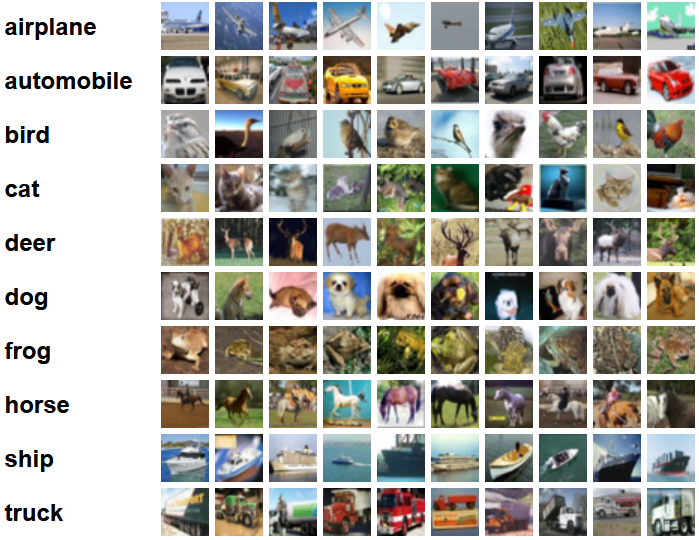
\includegraphics[width=0.6\textwidth]{MarcoTeorico/imgs/CIFAR-10.png}
    \caption{\textit{Dataset} CIFAR-10.}
    \label{fig:cifar10}
\end{figure}

Para todo aquel problema que implique separar un conjunto de datos en diferentes clases o categorías, sin importar el numero clases que pueden ser, se utiliza la clasificación.

\subsubsection{Regresión}

Los problemas de regresión predicen un valor real. En otras palabras, la función que estima la variable dependiente conociendo la variable independiente.

La regresión es utilizada para aquellos problemas que implican predecir valores numéricos, un ejemplo de esto son las predicciones de ráfagas de vientos las cuales dando como entrada diferentes características del ambiente podemos predecir la velocidad del viento.

\subsubsection{Regresión Lineal}

La clase más común de regresión es la regresión lineal. La regresión lineal intenta llegar a una función que describa la relación entre $x$ y $y$, para valores conocidos de $x$, predice valores de $y$ que resultan ser precisos (\cite{patterson2017deep}). La Figura \ref{fig:regresionLineal} representa la regresión en una gráfica.

\begin{figure}[H]
    \centering
    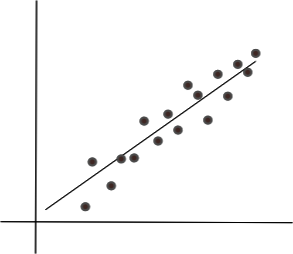
\includegraphics[width=0.5\textwidth]{MarcoTeorico/imgs/RegresionLineal.png}
    \caption{Grafica de regresión lineal.}
    \label{fig:regresionLineal}
\end{figure}

\subsubsection{Regresión Ridge}

La regresión Ridge es una versión regularizada de la regresión lineal, agrega un término de regularización en la función de costo (Ecuación \ref{eq:ridge}). Con esto se busca que el algoritmo mantenga los pesos lo más pequeños posible.

\begin{equation}
    \label{eq:ridge}
    \alpha \displaystyle\sum\limits_{i=1}^n (\theta_i)^{2}
\end{equation}

El hiperparametro $\alpha$ controla la regularización del modelo, si $\alpha = 0$ la regresión Ridge es simplemente una regresión lineal. Si $\alpha$ es muy grande, todos los pesos terminan igual a cero y resulta en una línea plana que pasa por la media de los datos(Figura \ref{fig:regresionRidge}.

\begin{figure}[H]
    \centering
    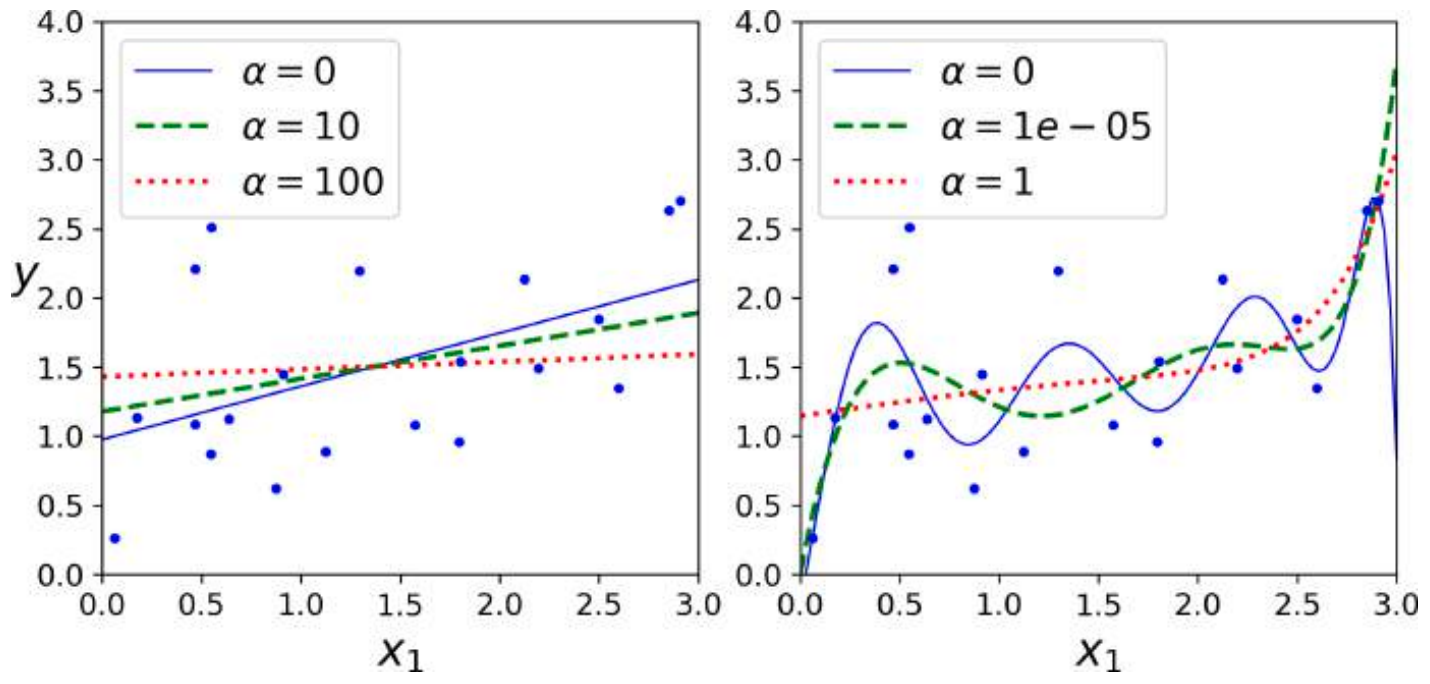
\includegraphics[width=0.8\textwidth]{MarcoTeorico/imgs/Ridge.png}
    \caption{Regresión Ridge con diferentes valores de $\alpha$.}
    \label{fig:regresionRidge}
\end{figure}

La Ecuación \ref{eq:ridgeCostFunction} es la función de costo para la regresión Ridge.

\begin{equation}
    \label{eq:ridgeCostFunction}
    J(\theta) = MSE(\theta)
    + \alpha \displaystyle\sum\limits_{i=1}^n (\theta_i)^{2}
\end{equation}

\subsubsection{Regresión Lasso}

La regresión Lasso (\textit{Least Absolute Shrinkage and Selection Operator} en Ingles) al igual que la regresión Ridge es una versión regularizada de la regresión lineal, sin embargo, la regresión Lasso utilizada valores absolutos en la función de regulación (Ecuación \ref{eq:lasso}), una característica importante con Lasso es que puede llegar a eliminar por completo los pesos de las características menos importantes.

\begin{equation}
    \label{eq:lasso}
    \alpha \displaystyle\sum\limits_{i=1}^n  \mid \theta_i \mid
\end{equation}

La Ecuación \ref{eq:lassoCostFunction} es la función de costo para la regresión Lasso.

\begin{equation}
    \label{eq:lassoCostFunction}
    J(\theta) = MSE(\theta)
    + \alpha \displaystyle\sum\limits_{i=1}^n  \mid \theta_i \mid
\end{equation}

\subsubsection{Elastic Net}

Elastic Net es una versión regularizada de la regresión lineal, siendo el punto medio entre la regresión Ridge y Lasso, utiliza un valor de regularización $r$, cuando $r = 0$ Elastic Net es equivalente a Ridge, y cuando $r = 1$, se comporta como Lasso (Ecuación \ref{eq:elasticNet}).

\begin{equation}
    \label{eq:elasticNet}
    r \alpha \displaystyle\sum\limits_{i=1}^n  \mid \theta_i \mid
    + \frac{1 - r}{2} \alpha \displaystyle\sum\limits_{i=1}^n  (\theta_i)^{2}
\end{equation}

La Ecuación \ref{eq:elasticNetCostFunction} es la función de costo para la regresión Elastic Net.

\begin{equation}
    \label{eq:elasticNetCostFunction}
    J(\theta) = MSE(\theta)
    + r \alpha \displaystyle\sum\limits_{i=1}^n  \mid \theta_i \mid
    + \frac{1 - r}{2} \alpha \displaystyle\sum\limits_{i=1}^n  (\theta_i)^{2}
\end{equation}

\subsection{Sobreajuste y Subajuste}

Cuando es entrenado un nuevo modelo se busca que tenga la capacidad de generalizar de tal manera que pueda interpretar datos de entrada que nunca haya visto.

Un buen modelo se equivoca poco en sus predicciones, esto significa que tiene un error bajo. Esto se evalúa ingresando al modelo datos que no recibió en su proceso de entrenamiento, de esta manera se tiene la seguridad de que el modelo es capaz de generalizar.

El subajuste ocurre cuando el modelo no puede obtener una pérdida suficientemente baja en el conjunto de entrenamiento. En este caso, el modelo no aprende los patrones en los datos de entrenamiento. Lo cual implica una gran cantidad de errores cuando es utilizado para realizar predicciones, como muestra la Figura \ref{fig:OverFiting}.


\begin{figure}[H]
    \centering
    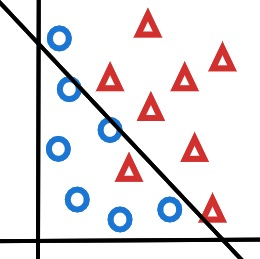
\includegraphics[width=0.4\textwidth]{MarcoTeorico/imgs/Ajuste_subajuste.jpg}
    \caption{Ejemplo de subajuste.}
    \label{fig:OverFiting}
\end{figure}


Por otro lado, tenemos un sobreajuste cuando la red modela los datos de entrenamiento demasiado bien y no se generaliza a los datos de validación (\cite{rosebrock2017deep}). En este caso tenemos que las predicciones solo serán buenas para aquellos que se utilice el mismo conjunto de datos que en el entrenamiento, Figura \ref{fig:underFiting}.

\begin{figure}[H]
    \centering
    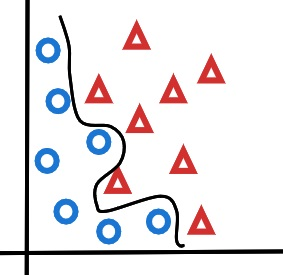
\includegraphics[width=0.4\textwidth]{MarcoTeorico/imgs/Ajuste_sobreajuste.jpg}
    \caption{Ejemplo de sobreajuste.}
    \label{fig:underFiting}
\end{figure}

Por otra parte, el entrenamiento ideal es cuando la red modela los datos de entrenamiento con cierto margen de error, pero siendo su gran mayoría correcta, Figura \ref{fig:idealFiting}.

\begin{figure}[H]
    \centering
    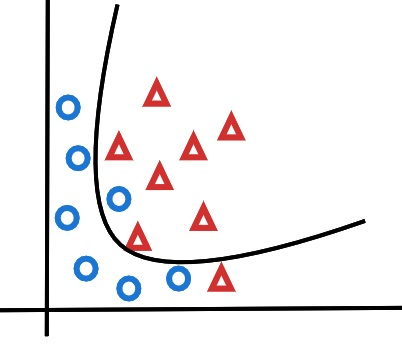
\includegraphics[width=0.6\textwidth]{MarcoTeorico/imgs/Ajuste_ideal.jpg}
    \caption{Ejemplo de ideal.}
    \label{fig:idealFiting}
\end{figure}

\subsection{Métricas de evaluación}


Ahora bien, cuando se realiza el entrenamiento es necesario saber que tan bueno es el modelo que se ha generado, para esto existen diferentes métricas que nos indican de manera cuantitativa la calidad del modelo.

Cuando se ha entrenado un modelo para un problema de clasificación se utilizan medidas de exactitud como una métrica de evaluación. La exactitud se calcula con el número de predicciones correctas entre el número de predicciones totales, La Ecuación \ref{eq:exactitud} muestra la métrica de exactitud.

\begin{equation}
    \label{eq:exactitud}
    Exactitud = \frac{Predicciones \: correctas}{ Total \: de \: predicciones}
\end{equation}

Por otra parte, los modelos creados para problemas de regresión hay tres métricas principales MAE, MSE Y RMSE.

La métrica de evaluación del Error Absoluto Medio (MAE – \textit{Mean Absolute Error} en Ingles) calcula la media de los valores absolutos de la diferencia entre los valores reales y los predichos. En otras palabras, MAE es el promedio de todos los errores sin tomar en cuenta si este error es positivo o negativo con respecto al valor real. La Ecuación \ref{eq:MAE} define el calculo de MAE.

\begin{equation}
    \label{eq:MAE}
    MAE = (\frac{1}{n}) \displaystyle\sum\limits_{i=0}^n \mid y_i - x_i \mid
\end{equation}

El Error Medio Cuadrado (MSE – \textit{Mean Square Error} en Ingles) se encarga de elevar al cuadrado el error, penalizando fuertemente los valores que se alejan demasiado del valor real esperado, con este valor se obtiene el promedio, la Ecuación \ref{eq:MSE} define el calculo de MSE.

\begin{equation}
    \label{eq:MSE}
    MSE = (\frac{1}{n}) \displaystyle\sum\limits_{i=0}^n (y_i - x_i)^{2}
\end{equation}

La Raíz del Error Cuadrático Medio (RMSE – \textit{Root Mean Square Error} en Ingles) al igual que la métrica MSE penaliza los errores altos, solo que para esta métrica se eliminan los cuadrados obteniendo la raíz del promedio obtenido con MSE. La Ecuación \ref{eq:RMSE} define el calculo de RMSE.

\begin{equation}
    \label{eq:RMSE}
    RMSE = \sqrt {
        (\frac{1}{n}) \displaystyle\sum\limits_{i=0}^n (y_i - x_i)^{2}
    }
\end{equation}

\section{Aprendizaje profundo}

\subsection{Redes neuronales}

Una red neuronal se llama así porque los científicos intentaron modelar el cerebro en código informático. El objetivo final es crear una “inteligencia general artificial”, en otras palabras un programa que puede aprender todo lo que una persona podria aprender.

Las redes neuronales artificiales son una clase de algoritmos de aprendizaje máquina que aprenden de los datos y se especializan en el reconocimiento de patrones (\cite{rosebrock2017deep}).

Una red neuronal es una función flexible que adapta de manera autónoma su comportamiento para satisfacer la relación entre la entradas y los resultados esperados y se ha denominado como un aproximador universal (\cite{goyal2018Deep}).

\subsection{Perceptrón}

Rosenblatt publicó el algoritmo seminal Perceptron: este modelo podía aprender automáticamente los pesos necesarios para clasificar una entrada.

Perceptron toma n entradas y produce una única salida binaria si la suma es mayor que el valor de activación. Se dice que la neurona se "dispara" siempre que se excede el valor de activación y se comporta como una función escalonada, lo cual se muestra en la ecuación \ref{eq:fnStep} (\cite{goyal2018Deep}).

\begin{equation}
\label{eq:fnStep}
    f\left(x\right)=\begin{cases}0 & x -u < 0\\1 & x -u >= 0\end{cases}
\end{equation}



Minsky y Papert demostraron que un perceptrón con una función de activación lineal es simplemente un clasificador lineal, incapaz de resolver problemas no lineales (\cite{rosebrock2017deep}). El ejemplo canónico de un problema no lineal es el conjunto de datos XOR Figura \ref{fig:xor}.

Perceptron se puede convertir fácilmente en un algoritmo en línea que procesa un flujo de ejemplos, actualizando el vector de peso solo si el último ejemplo recibido está mal clasificado. Se garantiza que el perceptrón convergerá en una solución si los datos de entrenamiento son linealmente separables, pero de lo contrario no convergerán(\cite{flach2012Machine}).

\begin{figure}[H]
    \centering
    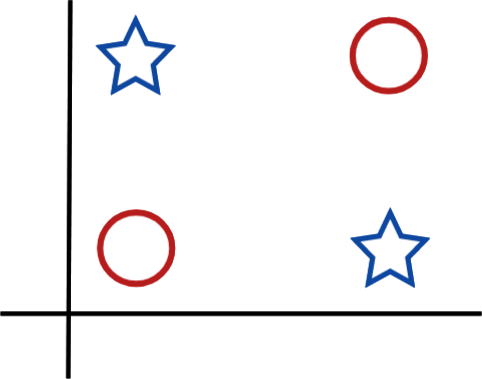
\includegraphics[width=0.5\textwidth]{MarcoTeorico/imgs/XOR.png}
    \caption{Problema XOR, no es linealmente separable.}
    \label{fig:xor}
\end{figure}


\subsection{Redes Neuronales Multicapa}


Los perceptrones multicapa o MLP (Multilayer Perceptron) son una red neuronal de propagación hacia adelante y se componen de múltiples perceptrones conectados entre sí y que operan en funciones de activación distintivas para permitir mejores mecanismos de aprendizaje. La arquitectura perceptrón multicapa cuenta como mínimo con 3 capas: una capa de entrada, una o más capas ocultas y una capa de salida (\cite{swamynathan2017Mastering}) Figura \ref{fig:mlp}.

\begin{figure}[H]
    \centering
    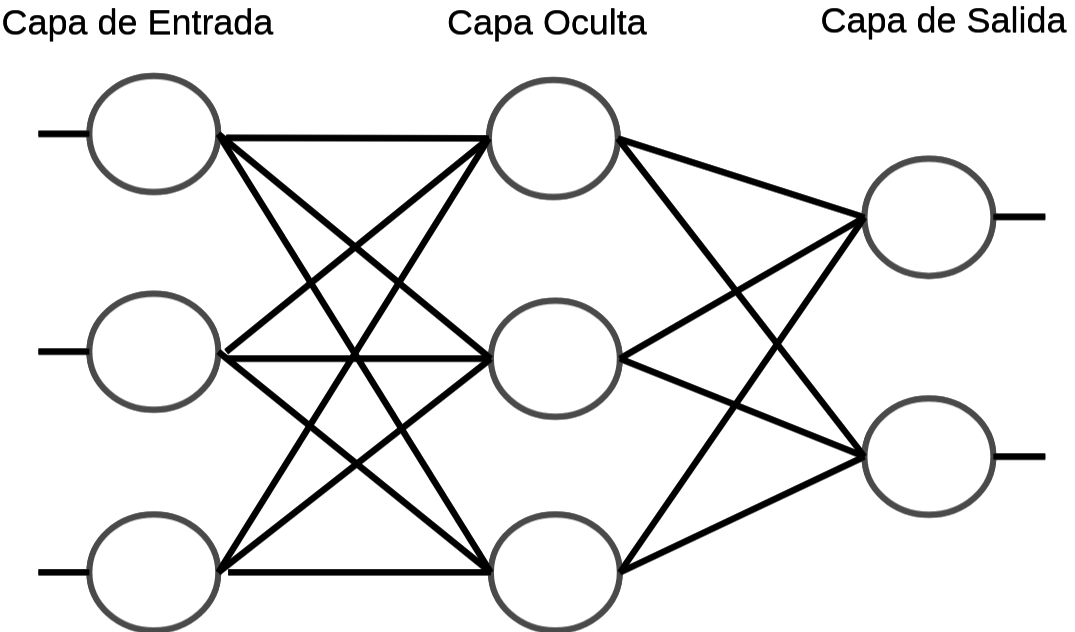
\includegraphics[width=0.5\textwidth]{MarcoTeorico/imgs/MLP.png}
    \caption{Representación básica de red neuronal multicapa.}
    \label{fig:mlp}
\end{figure}

Los MLP también se conocen como aproximadores universales, ya que pueden encontrar la relación entre los valores de entrada y los objetivos, utilizando una cantidad suficiente de neuronas en la capa oculta, alterando los pesos o utilizando datos de entrenamiento adicionales para aproximar la función dada hasta cualquier nivel de precisión. A menudo, con el grado de libertad dado a un MLP, puede superar a la red MLP básica, introduciendo más capas ocultas, con menos neuronas en cada una de las capas ocultas y pesos óptimos. Esto ayuda en el proceso de generalización general del modelo (\cite{goyal2018Deep}).

\subsection{Propagación hacia atrás(Backpropagation)}

En las redes neuronales es complicado ajustar sus pesos de entrenamiento por la gran cantidad de conexiones y sus múltiples niveles. Para lograr esta tarea, se utiliza el algoritmo backpropagation, creado por \citeauthor{rumelhart1986Parallel} en \citeyear{rumelhart1986Parallel}.

En el algoritmo Backpropagation calculamos qué tan rápido cambia el error a medida que cambiamos una capa oculta. A partir de ahí, podemos averiguar qué tan rápido cambia el error cuando cambiamos el peso de una conexión individual. Básicamente, intentamos encontrar el camino de descenso más empinado. Comenzamos calculando las derivadas del error con respecto a un solo ejemplo de entrenamiento. Una vez que tenemos las derivadas de error para una capa de unidades ocultas, las usaremos para calcular las derivadas de error para las unidades de la capa siguiente. Y una vez que encontramos las derivadas del error para las actividades de las unidades ocultas, es bastante fácil obtener las derivadas del error para los pesos que conducen a una unidad oculta (\cite{buduma2017Fundamentals}).

En resumen, el algoritmo backpropagation consiste en dos pasos como muestra la figura:

\begin{itemize}
\item Propagación hacia adelante: Se calculan los pesos de cada una de las neuronas, desde la capa de entrada hasta la capa de salida.

\item Propagación hacia atrás: Se calcula el error y se actualizan los pesos, desde la capa de salida hasta la capa de entrada.
\end{itemize}

\begin{figure}[H]
    \centering
    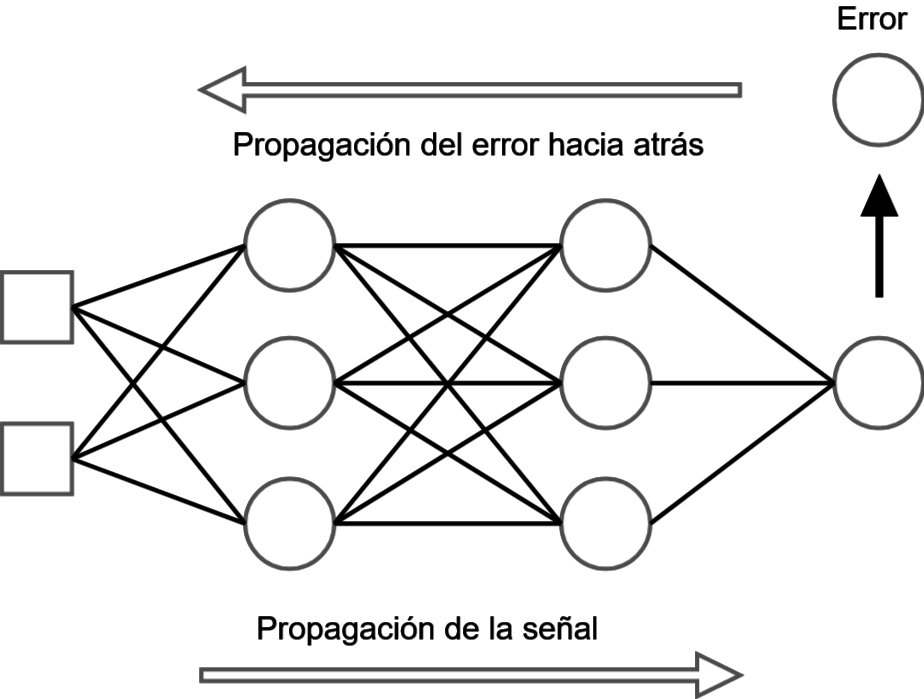
\includegraphics[width=0.8\textwidth]{MarcoTeorico/imgs/Backpropagation.png}
    \caption{Propagación hacia adelante y propagación hacia atrás.}
    \label{fig:backpropagation}
\end{figure}

\subsection{Descenso del Gradiente }

El método del descenso del gradiente es un algoritmo iterativo que minimiza una función de pérdida actualizando posteriormente los parámetros de la función.

\begin{figure}[H]
    \centering
    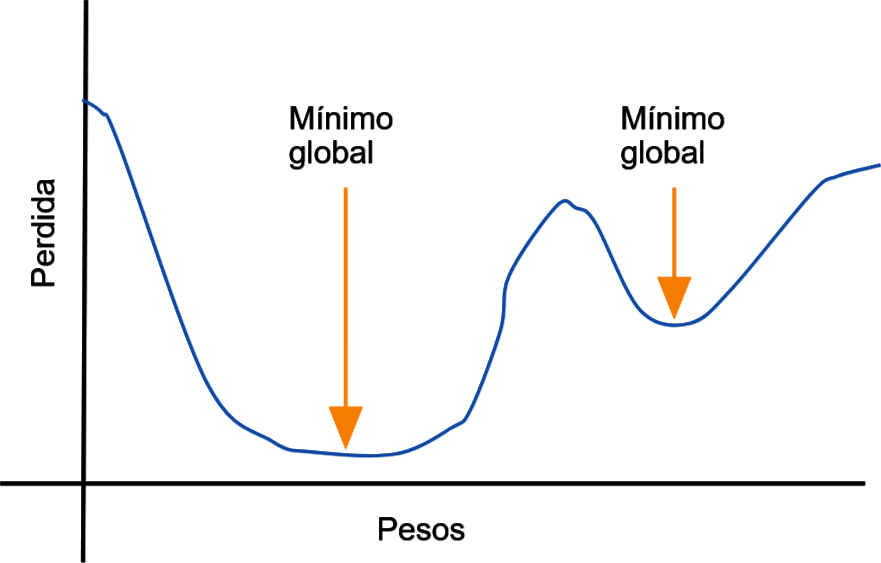
\includegraphics[width=0.8\textwidth]{MarcoTeorico/imgs/DescensoGradiente.png}
    \caption{Mínimo local y global.}
    \label{fig:descensoGradiente}
\end{figure}

La Figura \ref{fig:descensoGradiente} muestra cómo podemos tener múltiples picos y valles (Máximos y mínimos) para nuestros valores de perdida. El valor ideal que nos gustaría obtener es nuestro mínimo global, asegurando que nuestros parámetros tomen los valores más óptimos posibles.

El problema es que no tenemos una vista general en la que podamos encontrar de manera sencilla el mínimo global ya que en realidad nos colocaríamos en un lugar aleatorio sin saber dónde está el mínimo global y tendríamos que avanzar hacia una perdida mínima sin subir accidentalmente a la cima de un máximo local.

\subsection{Tasa de aprendizaje}

La tasa de aprendizaje es uno de los hiperparámetros más importantes. Tiene un fuerte impacto tanto en la estabilidad como en la eficiencia de los tiempos de entrenamiento y no hay una forma fija de encontrar la más adecuada. La tasa de aprendizaje es la magnitud del ajuste de pesos durante el entrenamiento de la red con el fin de minimizar el error (\cite{valenzuela2020Sistema}).

La imagen muestra que si la tasa es demasiado grande, nuestro entrenamiento es inestable. Si nuestra tasa de aprendizaje es demasiado pequeña, el entrenamiento puede tomar más tiempo para llegar a un entrenamiento adecuado.

\begin{figure}[H]
    \centering
    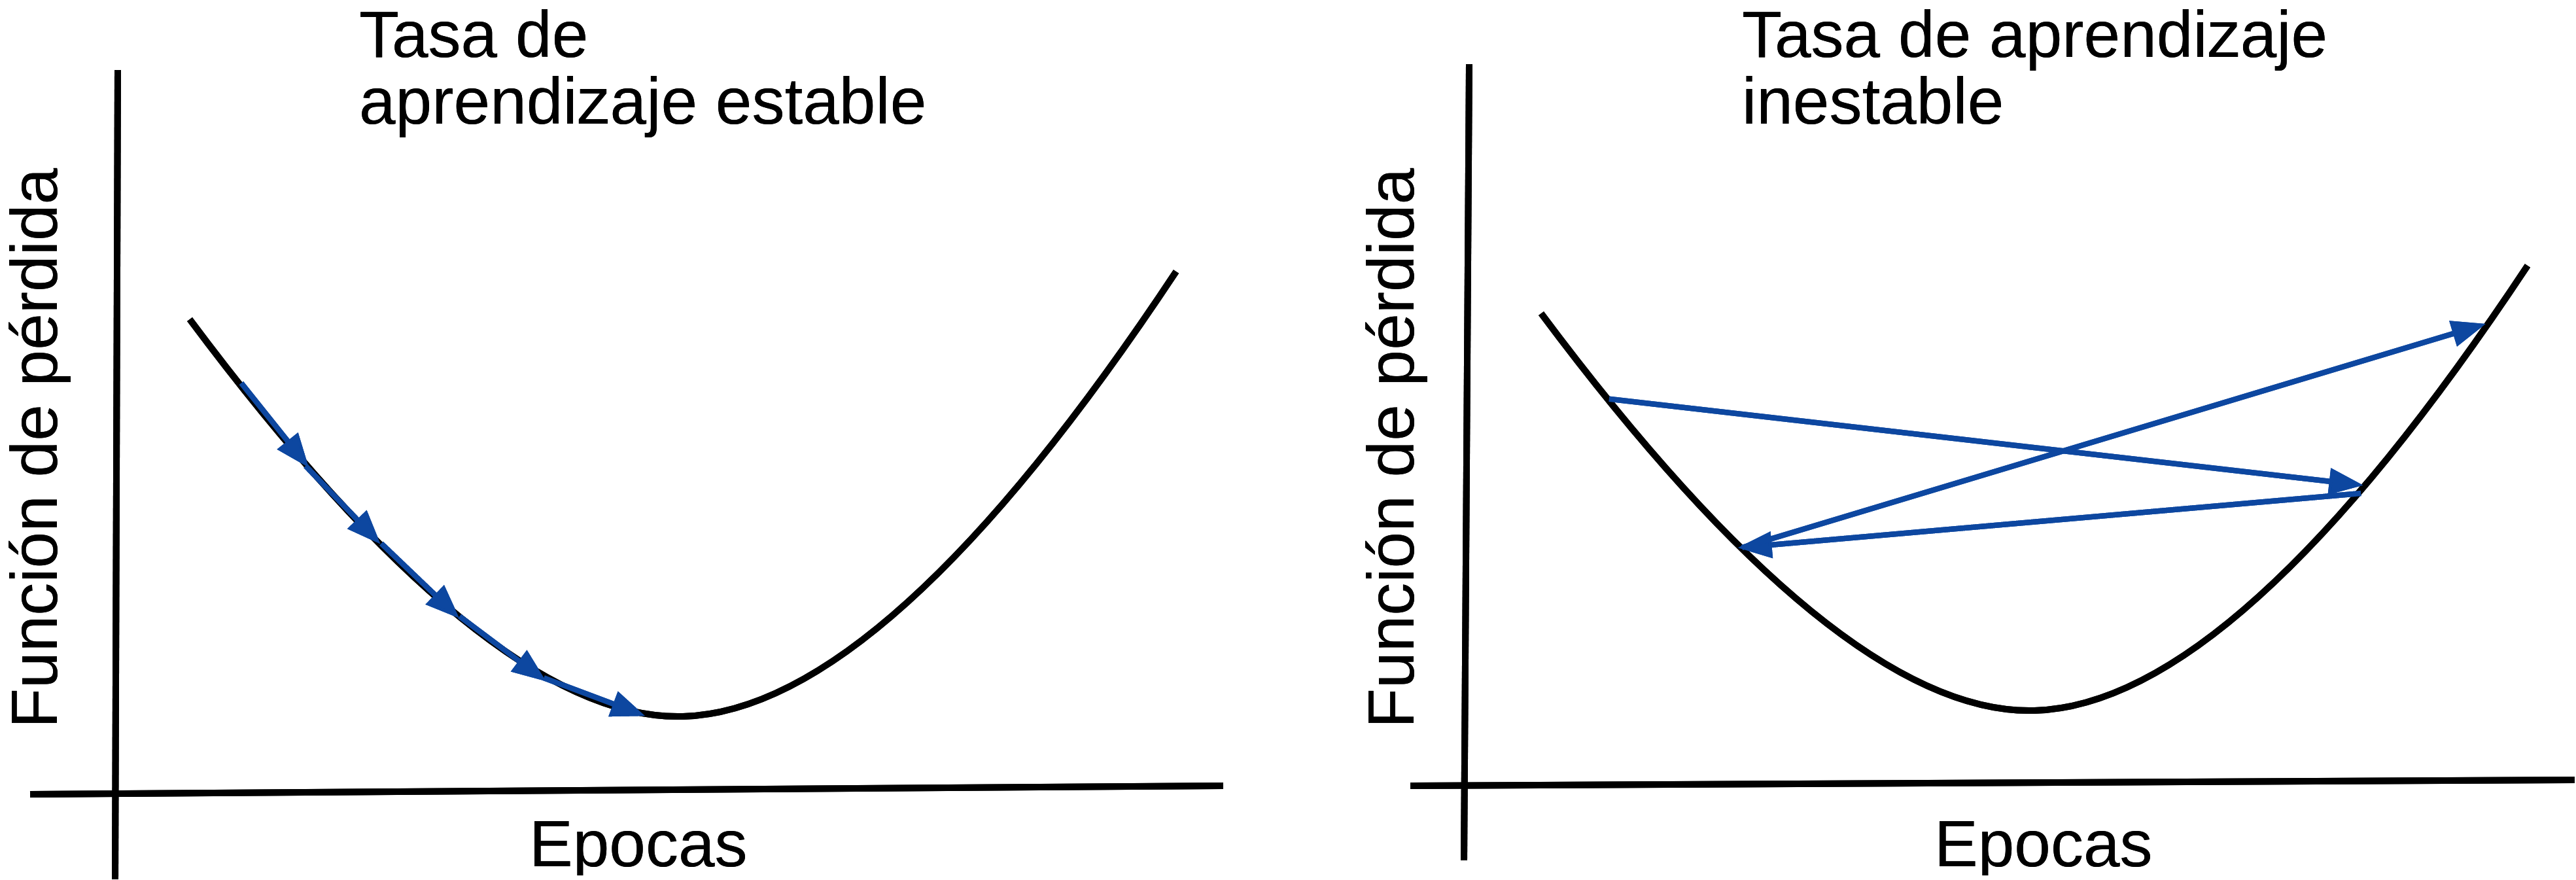
\includegraphics[width=0.8\textwidth]{MarcoTeorico/imgs/LearningRate.png}
    \caption{Tasa de aprendizaje.}
    \label{fig:learningRate}
\end{figure}

Preferiblemente, nuestra pérdida de entrenamiento y validación casi se imitan entre sí, con solo una pequeña brecha entre la pérdida de entrenamiento y la pérdida de validación, lo que indica un pequeño sobreajuste. Siempre que la brecha no aumente drásticamente, sabemos que existe un nivel aceptable de sobreajuste. Por otro lado, si no logramos mantener esta brecha y las pérdidas de entrenamiento y validación se separan drásticamente, entonces sabemos que corremos el riesgo de sobreajuste. Una vez que la pérdida de validación comienza a aumentar, sabemos que estamos muy sobreajustados (\cite{rosebrock2017deep}).


\subsection{Funciones de activación}

Las funciones de activación son una función de escalar a escalar, que produce la activación de la neurona. Usamos funciones de activación para propagar la salida de los nodos de una capa hacia la siguiente capa y para que las neuronas ocultas en una red neuronal para introducir la no linealidad del modelado de la red (\cite{patterson2017deep}).


Las funciones de activación definen el rango de valores que dará como resultado una de las capas de nuestra red neuronal, a partir de una función matemática.

\subsubsection{Función lineal}

La función lineal regresa como salida valores en el rango de $[-\infty,\infty]$ y está dada por la ecuación \ref{eq:linealFunc}:

\begin{equation}
\label{eq:linealFunc}
    f(x) = Wx
\end{equation}

\subsubsection{Sigmoidal}

La función sigmoidal nos da como salida valores en el rango de $[0,1]$ y está definida por la ecuación \ref{eq:sigmoidFunc}:

\begin{equation}
\label{eq:sigmoidFunc}
    s(x)={\frac {1}{1+e^{-x}}}
\end{equation}

\subsubsection{Tangente hiperbólica}

La función tangente hiperbólica proporciona como salida el rango $[-1,1]$ y está definida por la ecuación \ref{eq:tanhFunc}.

\begin{equation}
\label{eq:tanhFunc}
    \tanh (x)={\cfrac {e^{x}-e^{-x}}{e^{x}+e^{-x}}}
\end{equation}

\subsubsection{Softmax}

La función de activación softmax devuelve la distribución de probabilidad sobre clases de salida mutuamente excluyentes. La cual está definida por la siguiente ecuación \ref{eq:softmaxFunc}:

\begin{equation}
\label{eq:softmaxFunc}
  \sigma(\overrightarrow{z})_{i}=\frac{e^{z_{i}}}{
    \displaystyle\sum\limits_{j=1}^K e^{z_{j}}
  }
\end{equation}

donde $\overrightarrow{z}$ es el vector de entrada.

$z_i$ son los valores del vector de entrada.

$e^{z_{i}}$ es la función exponencial estándar que se aplica a cada elemento del vector de entrada.

$\displaystyle\sum\limits_{j=1}^K e^{z_{i}}$ es el término de normalización, asegura que todos los valores de salida de la función sumen 1 y cada uno esté en el rango $(0, 1)$, constituyendo así una distribución de probabilidad válida.

$k$ el numero de clases del clasificador multi-clases.

\subsubsection{ReLU}

La funcion Rectificador Lineal(ReLU) regresa como resultado valores en el rango de los números reales positivos $[0, \infty]$, como muestra la ecuación \ref{eq:reluFunc}:

\begin{equation}
\label{eq:reluFunc}
  relu(x)=\max(0,x)
\end{equation}


\subsection{Funciones de perdida}

Una función de pérdida indica la pérdida de predicción de $\hat{y}$ cuando la salida real es $y$. El objetivo del entrenamiento es entonces minimizar la pérdida en los diferentes ejemplos de entrenamiento. La función asigna una puntuación numérica a la salida de la red $\hat{y}$ dada la verdadera salida esperada $y$ (\cite{goldberg2017Neural}).

Dependiendo de nuestro problema es el tipo de función de perdida que usaremos. Para un problema de regresión se busca tener la perdida lo más cercana a cero y para un problema un problema de clasificación se busca tener el valor más algo o muy cercano a 1 para cada una de las clases para la cual fue entrenada nuestra red neuronal, siempre cuidando que la red neuronal no tenga sobreajuste claro.

Algunas de las funciones de perdida para problemas de  regresion son las siguientes:

\begin{itemize}
    \item Perdida de error cuadrático medio(MSE, \textit{Mean squared error loss})
    \item Perdida del error absoluto medio(MAE, \textit{Mean absolute error loss})
\end{itemize}

Mientras que para problemas de clasificación algunas de las funciones de perdida son las siguientes:

\begin{itemize}
    \item Perdida de bisagra
    \item Perdida logística
\end{itemize}

\subsection{Optimizadores}


\section{Tecnologías Utilizadas}

Para el desarrollo de este trabajo se utilizaron múltiples herramientas como lo son Git, SublimeText 3, Sublime Merge y los repositorios de Github todo bajo el sistema operativo Ubuntu 20.04.

A continuacion se presentan las herramientas de software de mayor impacto para el desarrollo de este trabajo.

\subsection{Python}

Python es un lenguaje de programación de alto nivel, interpretado y multipropósito. Python es muy utilizado por  la comunidad al ser un leguaje muy fácil de aprender y utilizar por ser un lenguaje de tipado dinámico, además de ser de código abierto.

Python ha tomado popularidad para el desarrollo en deep learning, por su facilidad de uso y la gran variedad de bibliotecas con las que cuenta como TensorFlow, PyTorch, Numpy, Scikit, entre otros.

\subsection{Contenedores Docker}

Un contenedor es una unidad de software que empaqueta el código y todas sus dependencias para que la aplicación se ejecute de forma rápida y confiable de un entorno informático a otro. Una imagen de contenedor de Docker es un paquete de software ligero, independiente y ejecutable que incluye todo lo necesario para ejecutar una aplicación: código, tiempo de ejecución, herramientas del sistema, bibliotecas del sistema y configuraciones \cite{docker2021container}.

La Figura \ref{fig:contenedorDocker} muestra las capas desde la infraestructura hasta los contenendores ejecutandose.

\begin{figure}[H]
    \centering
    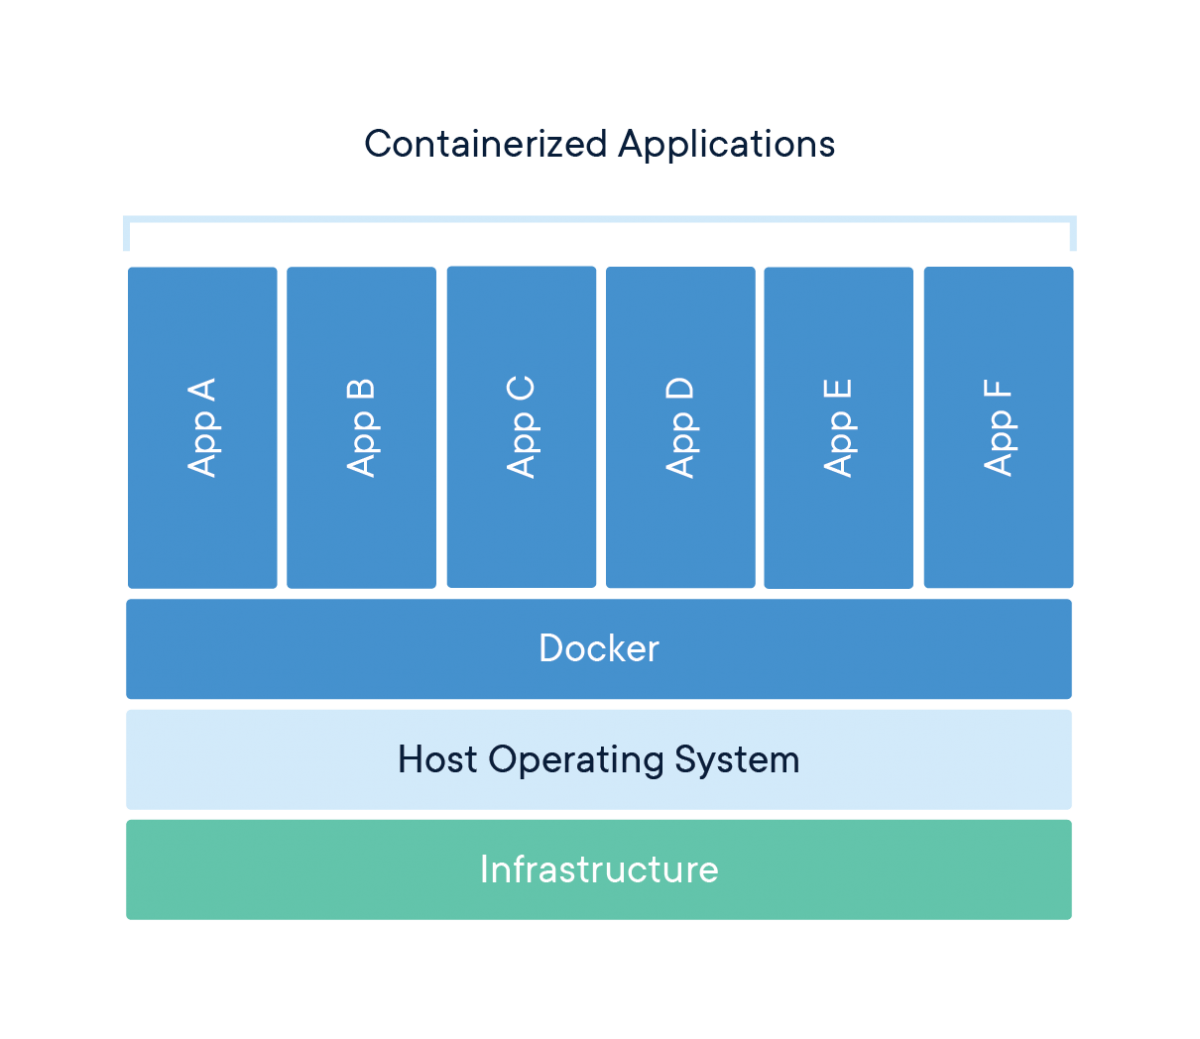
\includegraphics[width=0.6\textwidth]{MarcoTeorico/imgs/container-what-is-container.png}
    \caption{Representacion de un contenedor \cite{docker2021container}.}
    \label{fig:contenedorDocker}
\end{figure}


Docker fue la principal herramienta utilizada para el desarrollo de este trabajo, puesto que, sirvió para replicar múltiples trabajos del estado del arte sin necesidad de complicadas configuraciones al equipo utilizado, además de transferir los experimentos a otro equipo al solo utilizar la imagen creada para este experimento.

\subsection{Nvidia Docker}

NVIDIA Container Toolkit permite crear y ejecutar contenedores acelerados por GPU. Incluye una biblioteca de tiempo de ejecución de contenedores y utilidades para configurar automáticamente los contenedores para aprovechar las GPU de NVIDIA \cite{nvidiaDocker2021overview}.

Nvidia Docker permite la comunicación entre los contenedores de Docker y las GPU de Nvidia en la maquina utilizada como muestra la Figura \ref{fig:nvidiaDocker}.

\begin{figure}[H]
    \centering
    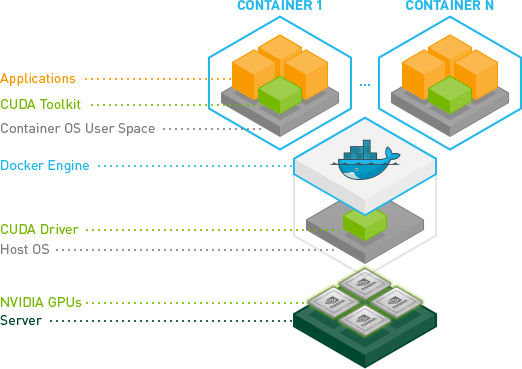
\includegraphics[width=0.6\textwidth]{MarcoTeorico/imgs/nvidia-docker.png}
    \caption{Arquitectura de Nvidia Docker \cite{nvidiaDocker2021overview}.}
    \label{fig:nvidiaDocker}
\end{figure}


\chapter{Estado del Arte}

Actualmente existen múltiples trabajos que determinan la velocidad de objetos, cada uno de una manera muy particular. En este capítulo se muestran algunos trabajos que se tomaron como referencia para desarrollar el presente trabajo.

\section{Determinación de velocidad con metodos de visión artificial}

Es posible determinar la velocidad y otras características usando las fórmulas físicas de cada una de ellas. Con lo cual podemos tener una respuesta rápida ya que no se necesita de mucho procesamiento para ejecutar estas fórmulas.

\citeauthor{singh2007Estimating} propone determinar la velocidad, aceleración y ángulo de un objeto en  una secuencia de imágenes. Para esto se deben cumplir con las siguientes características:

\begin{itemize}
\item Se conoce un rango aproximado de valores RGB del objeto.
\item Se conoce la velocidad a la que la cámara está tomando imágenes.
\item Se conoce aproximadamente el tamaño de la imagen.
\item La imagen es de color uniforme.
\item El fondo es de color uniforme y no es del color del objeto.
\end{itemize}

Para determinar los valores buscados se dibuja un punto en el centroide del objeto en la primera imagen y en la segunda imagen, a partir de tener los dos centroides es posible calcular la velocidad, aceleración y ángulo del objeto con las siguientes formulas:

\begin{eqnarray}
    \frac{
        \sqrt{
            (x2-x1)^{2} + (y2-y1)^{2}
        }
    }{
        FPS
    }\\
    \frac{
        v2-v1
    }{
        FPS
    }\\
    \tan^{-1}\frac{y2-y1}{x2-x1}
\end{eqnarray}


\citeauthor{anil2015Real} proponen un framework hibrido para el seguimiento de múltiples vehículos con la combinación del filtro Kalman y el algoritmo húngaro para resolver el problema de las obstrucciones. La estimación de la velocidad puede ser realizada sin la necesidad de calibrar las cámaras a utilizar, ya que utiliza las líneas del pavimento para realizar una estimación con un error máximo de 3 kilómetros por hora.


\citeauthor{li2014Video} desarrollan un sistema para recopilar datos de tráfico a partir de video, el sistema reconoce y se realiza el seguimiento de múltiples vehículos y sus velocidades medias. Propone la sustracción de fondo adaptativo basado en imágenes en color, se eliminan sombras y la configuración de la región de detección para mejorar la robustes del sistema. El conteo de vehículos tiene una precisión de 97.4\%, un error de clasificación de 8.3\% y un error absoluto de 2.3 kilómetros por hora.


\citeauthor{khan2019Multiple} proponen un sistema para realizar el seguimiento de vehículo y determinar el exceso de velocidad de vehículos. Para el seguimiento se aplica la diferenciación de cuadros para la detección de objetos. En la diferenciación de fotogramas, se calcula el modelo de fondo y el fotograma actual se resta del fotograma anterior, que se calcula durante el modelado. Después con el análisis de manchas se rastrean los objetos en la región de interés. El sistema propuesto tiene una precisión de 90\% para la detección y la medición de la velocidad.


\citeauthor{yang2019Vehicle} proponen el uso de cámaras estéreo calibradas con las cuales estiman la velocidad de vehículos. Este desarrollo usa un sistema optimizado Red de detectores multibox de un solo disparo que puede detectar de manera eficiente las matrículas en las dos vistas capturadas videos estéreo. El sistema funciona solo en el área de la placa, se calculan las coordenadas en un plano 3D correspondientes a los puntos de coincidencia estéreo. La velocidad se mide dividiendo la distancia entre dos puntos 3D por intervalo de cuadros. El sistema tiene un error de velocidad de –1.6 a +1.1 Km y una tasa de error máxima del 3.80\%.


\citeauthor{kamoji2020Image} proponen procesar un video cuadro a cuadro, en el cual cada cuadro se procesa con Image Enhancement para mejorar las características de la imagen, e vehículo se identifica con un cuadro delimitador aplicado al vehículo, para notar el movimiento en cada cuadro, el movimiento del vehículo se anota con cambio en el píxel y el cálculo de la velocidad se determina usando la fórmula de distancia considerando pixeles por metro.


\citeauthor{kurniawan2018Speed} proponen un sistema que puede monitorear la velocidad de algunos vehículos y determinar qué vehículos han superado la velocidad máxima permitida mediante el seguimiento del vehículo utilizando un método basado en coincidencias. Se utilizo el método de transformación proyectiva para calcular la velocidad de un vehículo. Este método se utiliza para transformar la imagen capturada en la imagen de la vista superior en forma de rectángulo. Según los resultados de las pruebas en el sistema a una velocidad de fotogramas de 30 FPS, la precisión de la velocidad de cálculo es del 97.01\% cuando no hay sombra y 83.86\% cuando hay sombra. Este sistema también puede determinar el tipo de vehículo de automóvil o motocicleta detectado que se rompe con una precisión del 89.62\%.


\citeauthor{peng2019Improved} determinan la velocidad de vehículos en movimiento con el uso de cámaras estéreos montadas en drones. Su método integra Mask-R-CNN  y K-Means con el algoritmo de pirámide Lucas Kanade. Mask-R-CNN se utiliza para reconocer los objetos que tienen movimientos en relación con el suelo y los cubre con máscaras para mejorar la similitud entre píxeles y reducir los impactos de los ruidosos píxeles en movimiento. Luego, se utiliza el algoritmo piramidal de Lucas Kanade para calcular el valor de flujo óptico. Finalmente, el valor es agrupado por el algoritmo K-Means para abandonar los valores atípicos, y la velocidad del vehículo es calculada por el flujo óptico procesado. En sus experimentos demuestran que el uso combinado de Lucas Kanade , Mask-R-CNN y K-Means, mejoran sus resultados en comparación del uso de estos métodos por separado o el uso combinado de solo 2 de ellos, aun habiendo realizado experimentos en circunstancias normales, con muchos objetos en movimiento y en circunstancias de poca luz.


\citeauthor{schoepflin2003Dynamic} nos muestran un algoritmo de 3 etapas para calibrar cámaras de tráfico en carretera y rastrear vehículos para crear un sensor de velocidad del tráfico. El algoritmo primero estima la posición de la cámara en relación a la carretera usando el movimiento y los bordes de los vehículos. Dada la posición de la cámara, el algoritmo calibra la cámara estimando los límites del carril y el punto de fuga de las líneas a lo largo de la carretera. El algoritmo transforma las coordenadas de la imagen del rastreador de vehículos en coordenadas del mundo real utilizando un modelo de cámara simplificado.


\citeauthor{yan2010Research} presenta un método de medición de la velocidad de vehículos en video y un análisis del error de la calibración de la cámara con el método Tsai de dos etapas. En primer lugar, los parámetros internos y externos de la cámara se obtuvieron según el método de dos etapas de Tsai. El desplazamiento del punto característico del mismo vehículo en cada imagen se extrajo y se convirtió al sistema de coordenadas mundiales. Por último, la velocidad de los vehículos se realizó con la diferencia de tiempo entre dos cuadros secuenciales. El resultado experimental muestra que el método de medición de la velocidad del vehículo no solo es simple y práctico, sino también muy robusto y preciso con un error cuadrático medio de 1.6273.


\citeauthor{luvizon2014Vehicle} nos muestran un sistema que utiliza la detección de texto para localizar las matrículas de los vehículos, la cual es utilizada para seleccionar las características más estables para el seguimiento. La velocidad del vehículo se estima comparando la trayectoria de las características rastreadas con medidas conocidas del mundo real. En los experimentos realizados las velocidades de los vehículos se estimaron con un error absoluto medio de 0.59 km/h.


\citeauthor{jalalat2016Vehicle} proponen la detección de vehículos y su velocidad con  un clasificador en cascada, basado en las características de Haar. Un algoritmo de segmentación de primer plano para distinguir los vehículos en movimiento del fondo y limpiar los resultados de detección para combinarlos con  resultados de seguimiento basados en el filtro Kalman y algoritmo de asignación de Munkres. Para lograr una medición de velocidad, se aplica una técnica eficiente de coincidencia de subpíxeles junto con un datos de visión estéreo para calcular los desplazamientos de vehículos por fotograma.


\citeauthor{llorca2016Two} determinan la velocidad de vehículos con el uso de dos cámaras montadas en un poste fijo. Usando diferentes distancias focales y orientaciones, cada cámara apunta a un tramo diferente de la carretera de unos pocos metros, lo que implica un escenario desafiante con la estimación de la distancia los errores deben ser del orden de centímetros.  El sistema propuesto determina la distancia relativa a los vehículos con respecto a las cámaras utilizando la placa como referencia demostramos que existe una geometría específica entre las cámaras que minimiza el error de velocidad. Los resultados obtenidos validan la propuesta con errores de velocidad máxima  de menos 3 k/h a velocidades de hasta 80 k/h.


\citeauthor{lee2021Study} desarrollaron un módulo para medir la distancia de vehículos en varios carriles simultáneamente usando un dron. El dron está montado con dos sensores LiDAR, y cada sensor emite un punto frontal y un punto trasero, donde los vehiculos son detectados. La velocidad del vehículo se estima utilizando la distancia entre el punto delantero y trasero por el cual pasa el vehículo y el tiempo que tarda en pasar por ambos puntos.


\citeauthor{yang2021Robust}, \citeauthor{yang2021Improved}, determinan la velocidad con cámaras estéreo que están ubicadas de fijas en un lugar estratégico de la ciudad. Las cámaras estéreo son las encargadas de identificar la matrícula, los faros y el logo, ya que estas se toman como las características principales ya que siempre aparecen en un vehículo; estas caracterisitcas se utilizan como referencia para determinar la velocidad. En \citeauthor{vakili2020Single}, se usa una estrategia similar identificando solo la placa como la caracteristica principal y usándola para determinar la velocidad del vehículo. Sin embargo, \citeauthor{vakili2020Single}, usa solamente una cámara, en lugar de cámaras estéreo.


\citeauthor{bevilacqua2016Egomotion} implementan la transformada de Hough para detectar las líneas carreteras para ser utilizadas como referencia. Para el seguimiento de los vehículos utilizan el popular algoritmo de Kanade-Lucas-Tomasi, para calcular la velocidad se determina la longitud de la región de interés en pixeles la cual equivale a la longitud en metros para después obtener la velocidad con respecto al tiempo en segundos.


\section{Redes neuronales para determinar velocidad y otras características}

Las redes neuronales pueden ser aplicadas para determinar la velocidad y otras características de objetos en movimiento obteniendo buenos resultados, hasta compararse con dispositivos especializados para esta tarea, sin embargo, esto implica mayor costo computacional para entrenar estas redes neuronales.


\citeauthor{bell2020Accurate} utilizan una cámara de video para estimar la velocidad vehicular. Con el uso de YOLOv2 se encargan de detectar los vehículos de la escena, mientras que el algoritmo de seguimiento en tiempo real en línea simple para el seguimiento de vehículos. La transformación del metraje de la cámara al Sistema de coordenadas de cuadrícula nacional británico, permitió la derivación de distancias del mundo real en la superficie plana de la carretera y las estimaciones simultáneas de la velocidad del vehículo. Las estimaciones lograron la raíz del error cuadrático medio y un error porcentual absoluto medio de 0.625 m/s y 20.922\%, respectivamente.


\citeauthor{dong2019Vehicle} proponen un método alternativo de extremo a extremo basado en redes convolucionales tridimensionales. El método propuesto basa la estimación de la velocidad promedio del vehículo en información de imágenes de video. El método se caracteriza por las siguientes tres características. Primero, el uso de bloques no locales en el modelo para capturar mejor la dependencia espacio-temporal de largo alcance. En segundo lugar, el uso de flujo óptico como entrada en el modelo. El flujo óptico incluye la información sobre la velocidad y la dirección del movimiento de los píxeles en una imagen. En tercer lugar, se construyó una red convolucional de múltiples escalas. Esta red extrae información sobre diversas características de los vehículos en movimiento. El método propuesto muestra resultados experimentales prometedores en un conjunto de datos de uso común con un error absoluto medio (MAE) de 2.71 km/h y un error cuadrático medio (MSE) de 14.62.


\citeauthor{burnett2020aUToTrack} presentan un nuevo conjunto de datos de detección y seguimiento de objetos (UofTPed50), que utiliza GPS para determinar la posición y velocidad de un peatón. Tambien presentan un sistema de seguimiento y detección de objetos liviano (aUToTrack) que utiliza visión, LIDAR y posicionamiento GPS/IMU para lograr un rendimiento de vanguardia en el punto de referencia de seguimiento de objetos de KITTI. Demostramos que aUToTrack estima con precisión la posición y la velocidad de los peatones, en tiempo real, utilizando solo CPU. Para poner a prueba el nuevo conjunto de entrenamiento UofTPed50 se utilizó la red SqueezeDet por contar con la característica de ser una de las redes más rápidas. Por otra parte para el seguimiento de objetos se utilizó el conjunto de entrenamiento KITTI con convoluciones rodantes recurrentes, ya que ocupa el primer lugar entre los trabajos publicados en el punto de referencia de detección de objetos 2D.


\citeauthor{kampelmuhler2018Camera} determinan la velocidad relativa de un vehículo utilizando una red neuronal perceptron multicapa la cual fue entrenada usando secuencias de imágenes, obteniendo buenos resultados con un error promedio de 1.12 m/s, el cual es comparable con un radar  LiDAR con un error de 0.71 m/s. Para determinar la velocidad se identificaron 3 características esenciales: la trayectoria del vehículo en un plano 2D, la profundidad y estimaciones de flujo óptico entre imágenes consecutivas. Al identificar un vehículo en una secuencia de imágenes podemos identificar que este, aumenta o disminuye su tamaño dependiendo la distancia que tiene con respecto al observador, esto complica el aprendizaje para la red neuronal por lo cual se opta por separar la información en cerca, medio y lejos, y entrenar un modelo para cada distancia.


\citeauthor{song2020Learning} determinan la velocidad y distancia de un vehículo usando dos fotogramas consecutivos, de los cuales obtienen las  características profundas, la geometría de la escena y el flujo óptico temporal. La arquitectura de esta red neuronal profunda se basó en la arquitectura de PWC-Net, la cual es una red de estimación de flujo óptico eficiente. Se extraen diferentes características de diferentes capas de la red para estimar la distancia y la velocidad del vehículo. En primer lugar, se presenta el modelo de regresión de distancia utilizando características profundas y geométricas espaciales de vehículos. Después de eso, se propone el método de estimación de la velocidad con características geométricas adicionales y una pista de flujo óptico temporal. Por último, detallan la canalización de la red centrada en vehículos para reducir la perspectiva y la influencia del movimiento.

\citeauthor{zhang2017Vehicle} realizaron experimentos para obtener la aceleración, la velocidad y la velocidad angular de un vehículo en movimiento usando cámaras de video posicionadas frente al área de interés. Para sus experimentos utilizaron el conjunto de datos KITTI el cual cuenta con imágenes estereoscópicas de la ciudad, así como arquitecturas CNN y la derivación y combinación de canales de entrada para identificar la dirección del flujo y las máscaras de objetos. Se creó una arquitectura CNN para cada característica buscada, aceleración, velocidad y velocidad angular. Se tomó como línea base una arquitectura CNN de 2 capas, que consta de 2 capas conv-relu-batchnorm-maxpooling y 2 capas afines-relu-batchnorm-dropout. Este proyecto compara los resultados para 4 arquitecturas CNN: línea de base, AlexNet, ResNet y AlexNet con el aprendizaje por transferencia.  Los resultados muestran que para el conjunto de entrenamiento ResNet tiene los mejores resultados seguido por AlexNet con el aprendizaje por transferencia, AlexNet y la línea base. Sin embargo, para el conjunto de validación  los mejores resultados los muestra la línea base, puesto que el entrenamiento de este modelo es más rápido y es posible buscar los hiperparametros para los mejores resultados. AlexNet con el aprendizaje por transferencia y AlexNet son los segundos mejores y ResNet tiene los peores resultados para el conjunto de validación.

\citeauthor{loor2017Visual} busca determinar la velocidad de los objetos utilizando 2 imágenes consecutivas. Para encontrar la velocidad el autor tomo como base la red neuronal FlowNet la cual ha aprendido a encontrar el flujo óptico en dos imágenes. FlowNet tiene dos arquitecturas de red diferentes: una arquitectura simple y una arquitectura de correlación. Ambas arquitecturas se basan en la red totalmente convolucional, lo que significa que esta red puede utilizar cualquier tamaño de imagen de entrada para determinar su flujo óptico. Una FlowNetSimple se entrena usando dos imágenes que se apilan juntas, dando lugar a una imagen de 6 dimensiones. Las siguientes capas se han diseñado como una red genérica, para permitir que la red decida cómo aprender el flujo óptico. En la FlowNetCorr se combinan las dos imágenes en una etapa posterior, después de que el modelo haya creado representaciones significativas de cada imagen por separado. Para ayudar al modelo a aprender las correspondencias entre la representación de características de las imágenes, se introdujo una capa de correlación. Para este trabajo se crearon 2 modelos basados en FlowNet, TimeNet y SpeedNet. TimeNet es un clasificador que puede predecir los tiempos entre fotogramas en milisegundos. SpeedNet es un modelo de regresión que genera una predicción de velocidad en forma de un solo valor. Tanto el modelo TimeNet como SpeedNet demostraron dar resultados aceptables cuando se tiene una velocidad baja, empeorando cuando la velocidad aumenta.

YOLO (\cite{redmon2016Yolo}) implementa la detección de objetos como un problema de regresión a cuadros delimitadores separados espacialmente y probabilidades de clase asociadas. Una sola red neuronal predice el área y las probabilidades de múltiples clases a partir de una imagen. Esto significa que YOLO razona globalmente sobre la imagen completa y todos los objetos de la imagen. Dado que toda la detección es una sola red, afecta directamente en el rendimiento de la detección. YOLO es implementada como una red neuronal convolucional y es evaluada usando el conjunto de datos PASCAL VOC. Las capas convolucionales iniciales de la red extraen características de la imagen, mientras que las capas completamente conectadas predicen las probabilidades y coordenadas de salida. Según los autores la red YOLO es extremadamente rápida lo cual la hace ideal para detecciones en tiempo real, procesando imágenes a 45 fotogramas por segundo. Una implementación reducida de la red puede procesar 155 fotogramas por segundo. Por otra parte, YOLO comete más errores de localización, al precio de disminuir la predicción de falsos positivos, superando otros métodos de predicción como DPM y RCNN.

\chapter{Metodología}
\label{cap:metodologia}

En este capítulo se describe el proceso de obtención de la velocidad de vehículos a partir de secuencias de imágenes. Para realizar esta tarea se recopiló un conjunto de datos (\textit{dataset}) suficiente para  realizar la tarea de estimación de la velocidad,  a partir del \textit{dataset}. El problema de obtención de la velocidad fue dividido en tres procesos principales (extracción de características, modelo predictivo y obtención de la velocidad). Para la generación del \textit{dataset} fue necesario ir físicamente a una vía terrestre. Una vez en la vialidad, se utilizó una cámara para capturar la secuencias de imágenes y un radar para medir la velocidad del vehículo. El proceso de extracción de características parte de los videos (secuencias de imágenes) para después aplicar técnicas de aprendizaje profundo. Resultando en un archivo con extensión csv con las características esenciales con los vehículos en cuestión. A partir del archivo con extensión csv se aplicaron técnicas estadísticas de correlación con la finalidad de relacionar la distancia en píxeles con una distancia en metros. Para posteriormente estimar la velocidad del vehículo (obtención de la velocidad). 


La metodología completa se divide en dos grandes procesos como lo muestra la Figura \ref{fig:MetodologiaDF}. El proceso de obtención del conjunto de datos, que consistió en la generación de muestras de campo con las cuales se realizó esta investigación. Y a partir de las muestras recolectadas se realizó el proceso de obtención de la velocidad.

\begin{figure}[H]
    \centering
    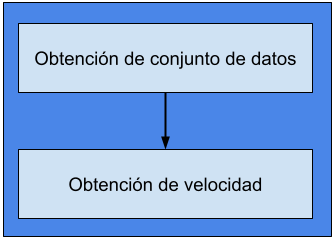
\includegraphics[width=0.5\textwidth]{Metodologia/imgs/ProcesoObtencionVelocidad.png}
    \caption{Proceso de obtención de la velocidad.}
    \label{fig:MetodologiaDF}
\end{figure}


\section{Obtención de conjunto de datos}


La obtención del conjunto de datos se divide en dos etapas, la primera etapa corresponde a la toma de muestras, la cual implica ir al lugar con flujo constante de vehículos para obtener la mayor cantidad de datos. La segunda etapa es la limpieza de las muestras con la cual se busca solo tomar en cuenta los vehículos a los que se logró tomar correctamente la velocidad.
La Figura \ref{fig:DFCreacionCD} muestra las dos etapas internas con las que cuenta la obtención de conjunto de datos.

\begin{figure}[H]
    \centering
    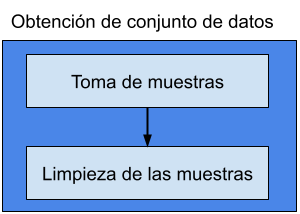
\includegraphics[width=0.5\textwidth]{Metodologia/imgs/ObtencionConjuntoDatos.png}
    \caption{Proceso de obtención de conjunto de datos.}
    \label{fig:DFCreacionCD}
\end{figure}


%%%%%%%%%%%%%%%%%%%%%%%%%%%%%%%%%%%%%%%%%%%%%%%%%%%%%%%%%%%%%%%%%%%%%%%%%%%%%%%%
%%%%%%%%%%%%%%%%%%%%%%%%%%%%%%%%%%%%%%%%%%%%%%%%%%%%%%%%%%%%%%%%%%%%%%%%%%%%%%%%
%%%%%%%%%%%%%%%%%%%%%%%%%%%%%%%%%%%%%%%%%%%%%%%%%%%%%%%%%%%%%%%%%%%%%%%%%%%%%%%%
%%%%%%%%%%%%%%%%%%%%%%%%%%%%%%%%%%%%%%%%%%%%%%%%%%%%%%%%%%%%%%%%%%%%%%%%%%%%%%%%
%%%%%%%%%%%%%%%%%%%%%%%%%%%%%%%%%%%%%%%%%%%%%%%%%%%%%%%%%%%%%%%%%%%%%%%%%%%%%%%%

\subsection{Toma de muestras}

Para la toma de muestras se requirió de dos dispositivos con los cuales se busca la extracción del conjunto de datos que posteriormente se utilizará como entrenamiento de los modelos predictivos. Uno de los dispositivos es el radar Bushnell (Figura \ref{fig:RadarVelocidad}) el cual tiene una precisión de +/- 1.6 kilómetros por hora.

\begin{figure}[H]
    \centering
    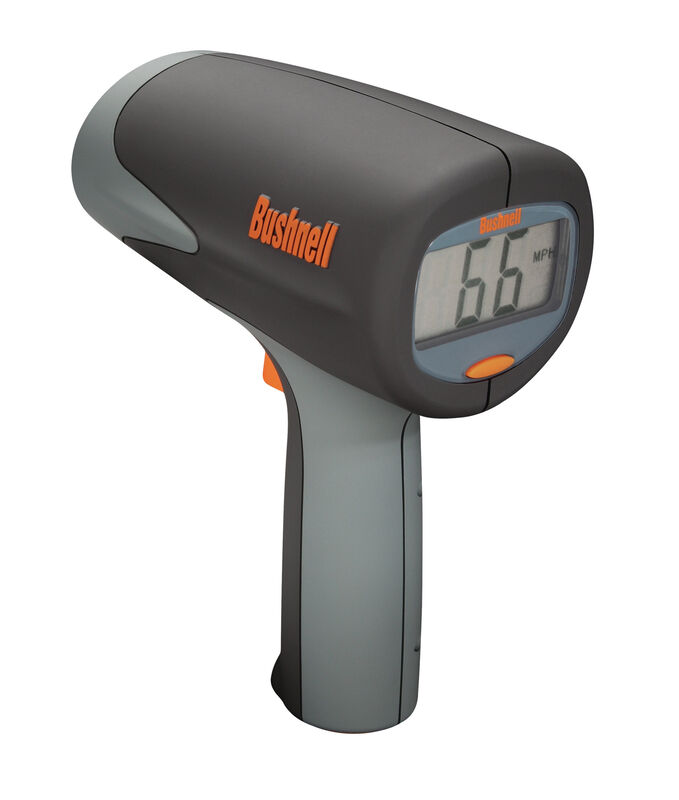
\includegraphics[width=0.4\textwidth]{Metodologia/imgs/bushnell.jpg}
    \caption{Radar de velocidad Bushnell(\cite{bushnell}).}
    \label{fig:RadarVelocidad}
\end{figure}

Mientras que el otro dispositivo es una cámara de video, la cual puede ser un dispositivo especializado para esta tarea o cualquier otro dispositivo capaz de grabar video. 
Las configuraciones mínimas pueden ser una resolución de 854 x 480 a 30 fotogramas por segundo. Sin embargo, hay que tomar en cuenta que al tener una resolución baja se puede perder calidad en la imagen y tomar un área menor a la deseada. Mientras que tener fotogramas tan bajos ocasionará perder vehículos que pasan a una velocidad más alta.
Por otro parte al aumentar la resolución y los fotogramas por segundo ocasiona que al sistema le tome más tiempo procesar el video. Para este caso se utilizó la cámara de Smartphones un Xiaomi Redmi Note 7 y un iPhone X configurados a 60 FPS y una resolución de Full HD (1920 x 1080 pixeles).

Existe un cuidado especial a la hora de posicionar la cámara, ya que no se quiere que los experimentos sean considerados como cálculos de velocidad en 2D, para esto la toma de muestras se realizó en un lugar donde el tráfico vehicular pase con cierto grado de inclinación, sin apuntar la cámara directamente al costado de donde pasan los vehículos, como muestra la Figura \ref{fig:LugarMuestrasDataset}.

\begin{figure}[H]
    \centering
    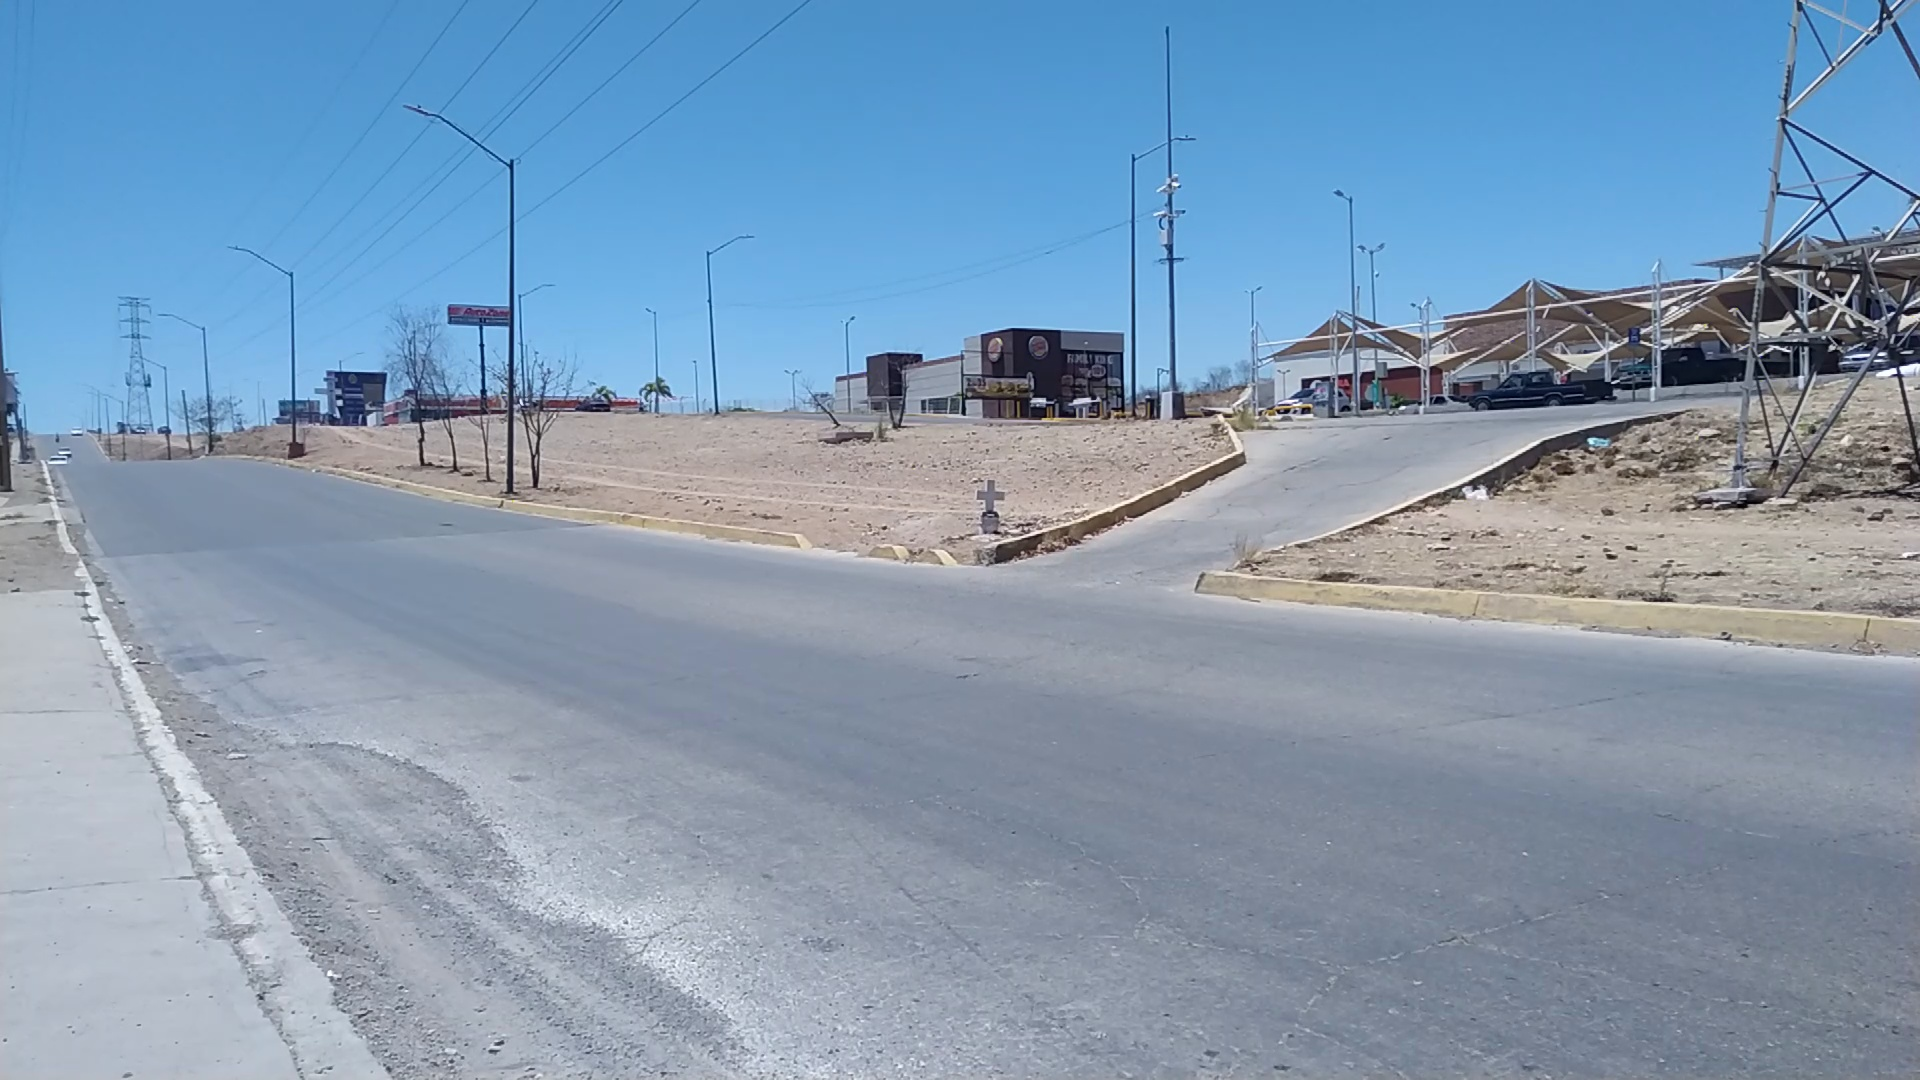
\includegraphics[width=0.8\textwidth]{Metodologia/imgs/LugarMuestras.jpg}
    \caption{Lugar donde se tomaron las muestras.}
    \label{fig:LugarMuestrasDataset}
\end{figure}

Cabe mencionar que por practicidad, el proceso de toma de muestras fue realizado, en un mismo lugar de la ciudad de Culiacán, Sinaloa.

Dado que la cámara y el radar de velocidad son dispositivos que no están sincronizados entre sí, fue necesario la implementación de un mecanismo para asociar la lectura del radar con la toma del video.

%%%%%%%%%%%%%%%%%%%%%%%%%%%%%%%%%%%%%%%%%%%%%%%%%%%%%%%%%%%%%%%%%%%%%%%%%%%%%%%%
%%%%%%%%%%%%%%%%%%%%%%%%%%%%%%%%%%%%%%%%%%%%%%%%%%%%%%%%%%%%%%%%%%%%%%%%%%%%%%%%
%%%%%%%%%%%%%%%%%%%%%%%%%%%%%%%%%%%%%%%%%%%%%%%%%%%%%%%%%%%%%%%%%%%%%%%%%%%%%%%%
%%%%%%%%%%%%%%%%%%%%%%%%%%%%%%%%%%%%%%%%%%%%%%%%%%%%%%%%%%%%%%%%%%%%%%%%%%%%%%%%
%%%%%%%%%%%%%%%%%%%%%%%%%%%%%%%%%%%%%%%%%%%%%%%%%%%%%%%%%%%%%%%%%%%%%%%%%%%%%%%%

\subsection{Limpieza de las muestras}

Una vez tomadas las muestras, fue necesario realizar una limpieza de los datos, estos son, los vehículos a los que se les detectó la velocidad utilizando el radar. Con la limpieza de los datos se busca eliminar los vehículos a los que no se les tomo la velocidad y dejando solo aquellos que si fueron considerados.

La toma de las muestras se realizá a partir de dos dispositivos que no están especializados para esta tarea (Cámara de video y radar de velocidad), la limpieza de las muestras ayuda a combinar la información de ambos dispositivos realizando una inspección visual de los videos, en la cual se identifica el segundo del video en el que pasa el vehículo de interes, la velocidad detectada por el radar, el carril por el cual viaja el vehículo y una descripción del vehículo para futuras referencias. Estos cuatro datos son guardados en un archivo de texto separado por comas (csv) el cual servirá de entrada para el siguiente paso en la metodología.

Determinar la velocidad es una tarea que necesita el tiempo y la distancia que toma un vehículo en pasar de un lugar a otro. Para esto el sistema necesita ser configurado con un punto de entrada y un punto de salida en el eje X. A partir de ahora a estos dos puntos se les llamará simplemente por punto A y punto B.  Los puntos A y B deben ser colocados de manera que los vehículos deben pasar completamente por cada uno de ellos. Además, cada una de las muestras deben tener diferentes valores para los puntos A y B, sin embargo, para este caso no fue necesario implementar diferentes valores, ya que todos los videos fueron tomados en el mismo lugar. La Figura \ref{fig:LugarLimites} muestra donde fueron colocados los puntos A y B en las muestras, denotados por dos lineas azules verticales.

\begin{figure}[H]
    \centering
    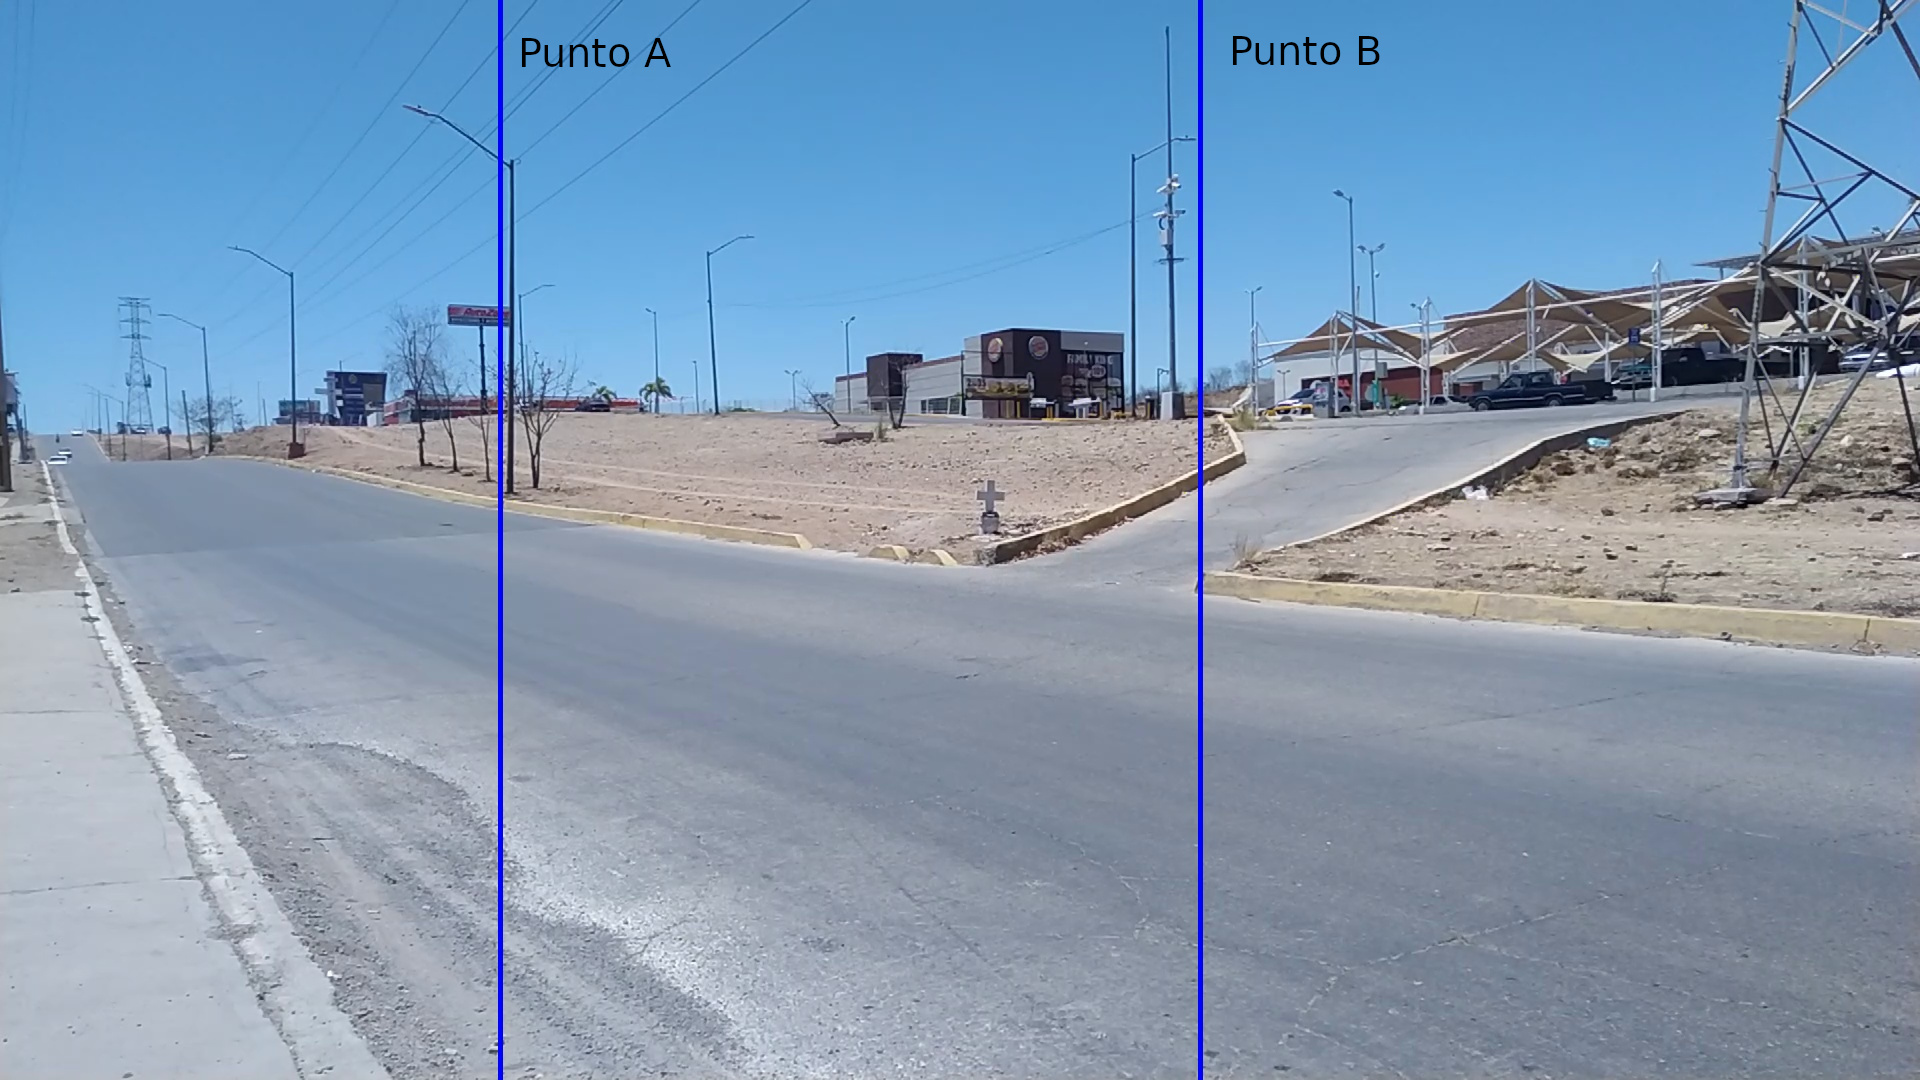
\includegraphics[width=0.8\textwidth]{Metodologia/imgs/LugarLimites_01.jpg}
    \caption{Límites para lugar de las muestras.}
    \label{fig:LugarLimites}
\end{figure}

Una vez que se deciden los valores para los puntos A y B, se genera el archivo csv. Para esto se toma en cuenta el segundo en que pasa debe ser lo más cercano posible al centroide del vehículo cuando pasa por el punto B. Es importante ingresar una descripción, aunque esta no va a ser usada por el sistema. Se volverá importante para validar que el vehículo al que se le tomó la velocidad es el mismo que detecto el sistema.

%%%%%%%%%%%%%%%%%%%%%%%%%%%%%%%%%%%%%%%%%%%%%%%%%%%%%%%%%%%%%%%%%%%%%%%%%%%%%%%%
%%%%%%%%%%%%%%%%%%%%%%%%%%%%%%%%%%%%%%%%%%%%%%%%%%%%%%%%%%%%%%%%%%%%%%%%%%%%%%%%
%%%%%%%%%%%%%%%%%%%%%%%%%%%%%%%%%%%%%%%%%%%%%%%%%%%%%%%%%%%%%%%%%%%%%%%%%%%%%%%%
%%%%%%%%%%%%%%%%%%%%%%%%%%%%%%%%%%%%%%%%%%%%%%%%%%%%%%%%%%%%%%%%%%%%%%%%%%%%%%%%
%%%%%%%%%%%%%%%%%%%%%%%%%%%%%%%%%%%%%%%%%%%%%%%%%%%%%%%%%%%%%%%%%%%%%%%%%%%%%%%%

\section{Obtención de velocidad}

Como se mencionó anteriormente en la Sección \ref{cap:metodologia} la obtención de la velocidad se divide en tres partes las cuales están representadas en el Figura \ref{fig:DFObtencionDeVelocidad} y se describen a continuación.

\begin{figure}[H]
    \centering
    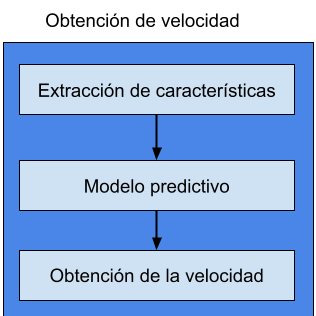
\includegraphics[width=0.5\textwidth]{Metodologia/imgs/ObtencionVelocidad.png}
    \caption{Proceso de obtención de velocidad.}
    \label{fig:DFObtencionDeVelocidad}
\end{figure}

\subsection{Extracción de características }

En el paso anterior para cada muestra se creo un archivo csv el cual servirá de entrada para el paso actual.

El sistema se encarga de leer el video utilizando la biblioteca OpenCV con la cual se extraen los fotogramas del video, cada fotograma pasa por la red neuronal YOLO la cual se encarga de identificar todos los vehículos que aparecen en el fotograma. YOLO regresa las coordenadas de cada objeto detectado dentro del fotograma, estas coordenadas son usadas para dibujar un recuadro para cada objeto. La Figura \ref{fig:LugarDeteccion} muestra dos vehículos detectados.

\begin{figure}[H]
    \centering
    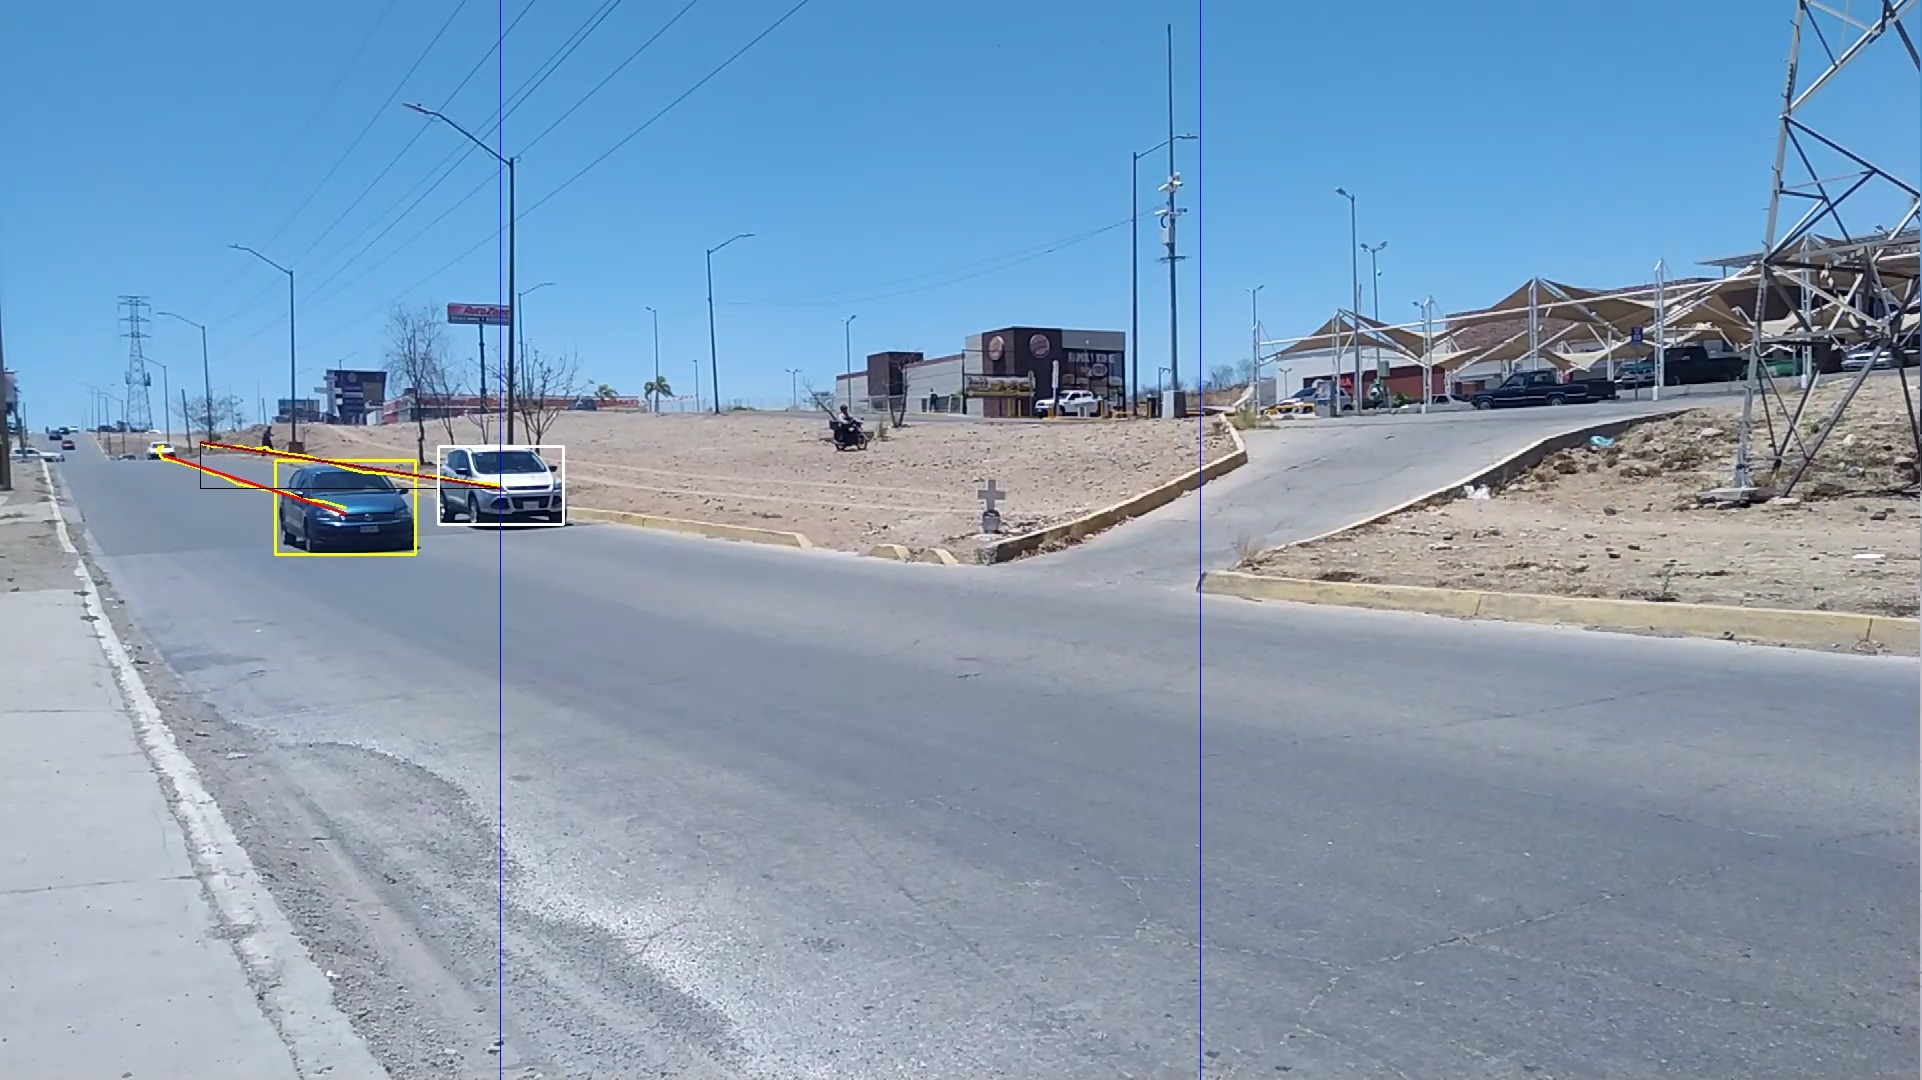
\includegraphics[width=0.8\textwidth]{Metodologia/imgs/Deteccion.jpg}
    \caption{Detección de vehículos dentro de recuadros.}
    \label{fig:LugarDeteccion}
\end{figure}

El seguimiento de los vehículos se realiza por medio del Filtro Kalman el cual determina su ubicación en el próximo fotograma. El sistema se encarga de guardar todas las ubicaciones de los vehículos en el transcurso del tiempo siendo capaz dibujar todo el trayecto que han tenido cada uno de ellos. Sumando el uso de regresión lineal se crea una recta que corresponde a las trayectorias de los vehículos. La Figura \ref{fig:LugarSeguimiento} muestra un vehículo detectado en un recuadro blanco, una línea amarilla con la trayectoria del vehículo y una línea roja la cual es generada con regresión a partir de la trayectoria del vehículo.

\begin{figure}[H]
    \centering
    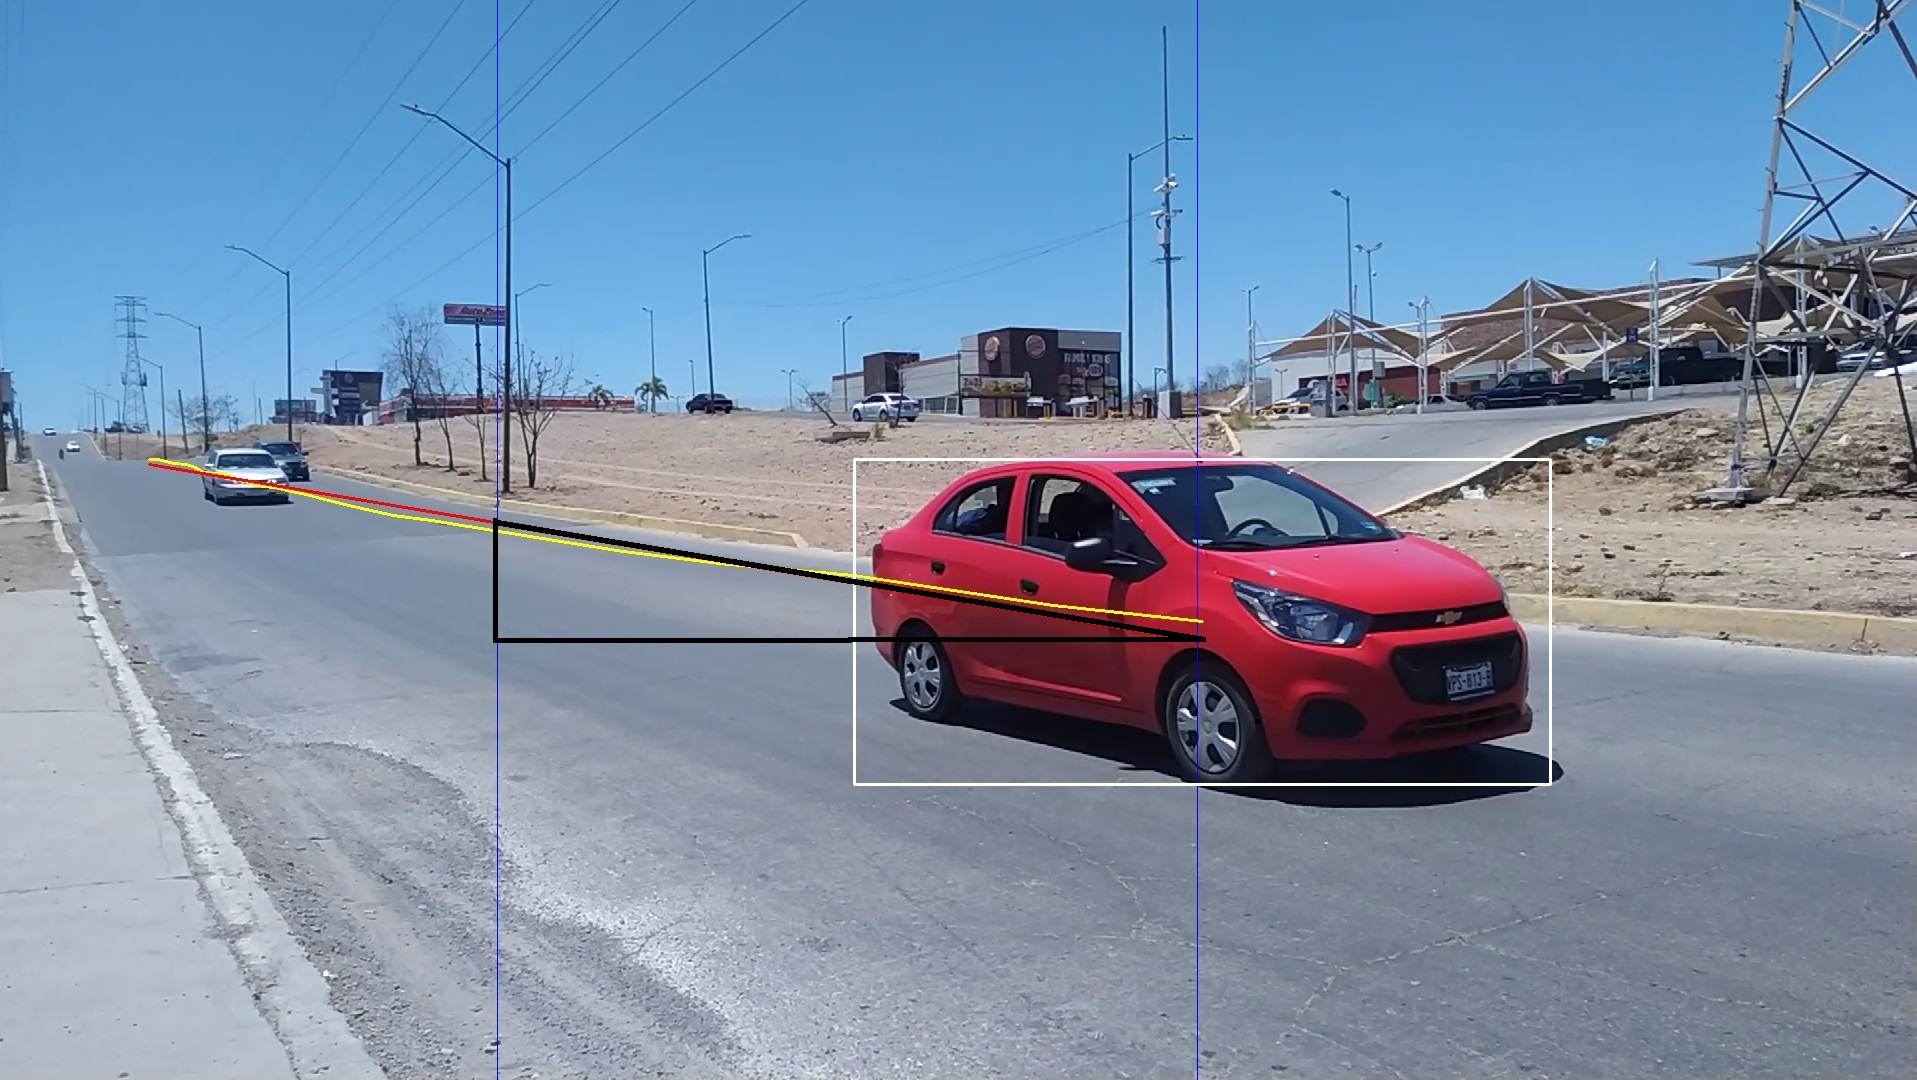
\includegraphics[width=0.8\textwidth]{Metodologia/imgs/Seguimiento_01.jpg}
    \caption{Detección de vehículos en punto B, sus trayectorias y triangulación del generado con el punto A y B.}
    \label{fig:LugarSeguimiento}
\end{figure}

Otra característica que se identifica en la Figura \ref{fig:LugarSeguimiento} es la creación de un triángulo en color negro, con el cual se identifica el ángulo detectado para el vehículo.

Cando el sistema detecta que un vehículo pasa por el punto A, este guarda la información del estado del vehículo (Figura \ref{fig:PuntoA}). Puede haber múltiples vehículos pasando en ese momento y todos serán detectados por el sistema. El vehículo del cual se obtienen sus características esta identificado con un recuadro de color amarillo, mientras que el resto de los vehículos están dentro de un recuadro color amarillo.


\begin{figure}[H]
    \centering
    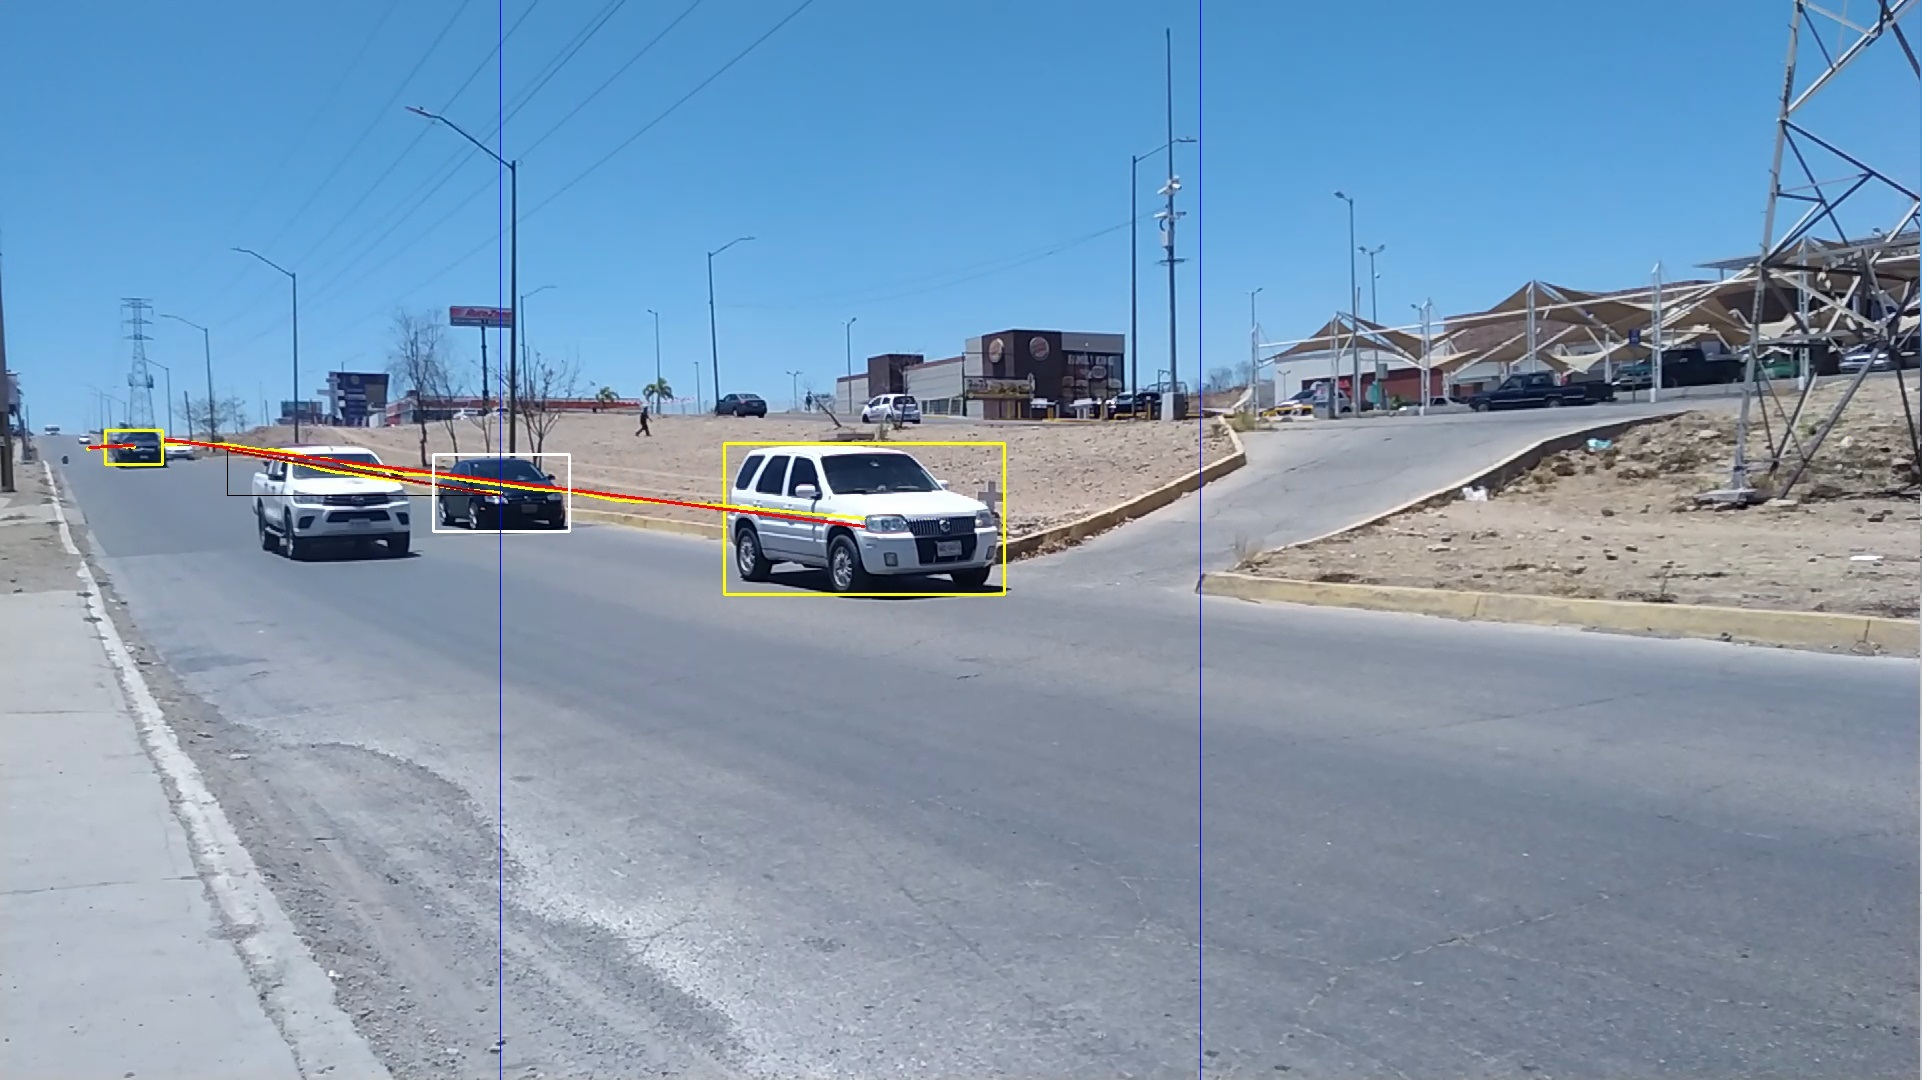
\includegraphics[width=0.8\textwidth]{Metodologia/imgs/Punto_A.jpg}
    \caption{Punto A con vehículo en recuadro blanco.}
    \label{fig:PuntoA}
\end{figure}

Aunque se guardó el estado del vehículo cuando paso por el punto A, este no genera una línea para el archivo csv resultante. Es hasta que el vehículo pasa por el punto B y coincide con los segundos en el archivo csv de entrada que el sistema guarda un nuevo dato en el archivo de salida. Los vehículos que no cuentan con una línea en el archivo csv de entrada no se les guarda su información. La Figura \ref{fig:PuntoB} muestra cuando el vehículo detectado en el punto A pasa por el punto B.

\begin{figure}[H]
    \centering
    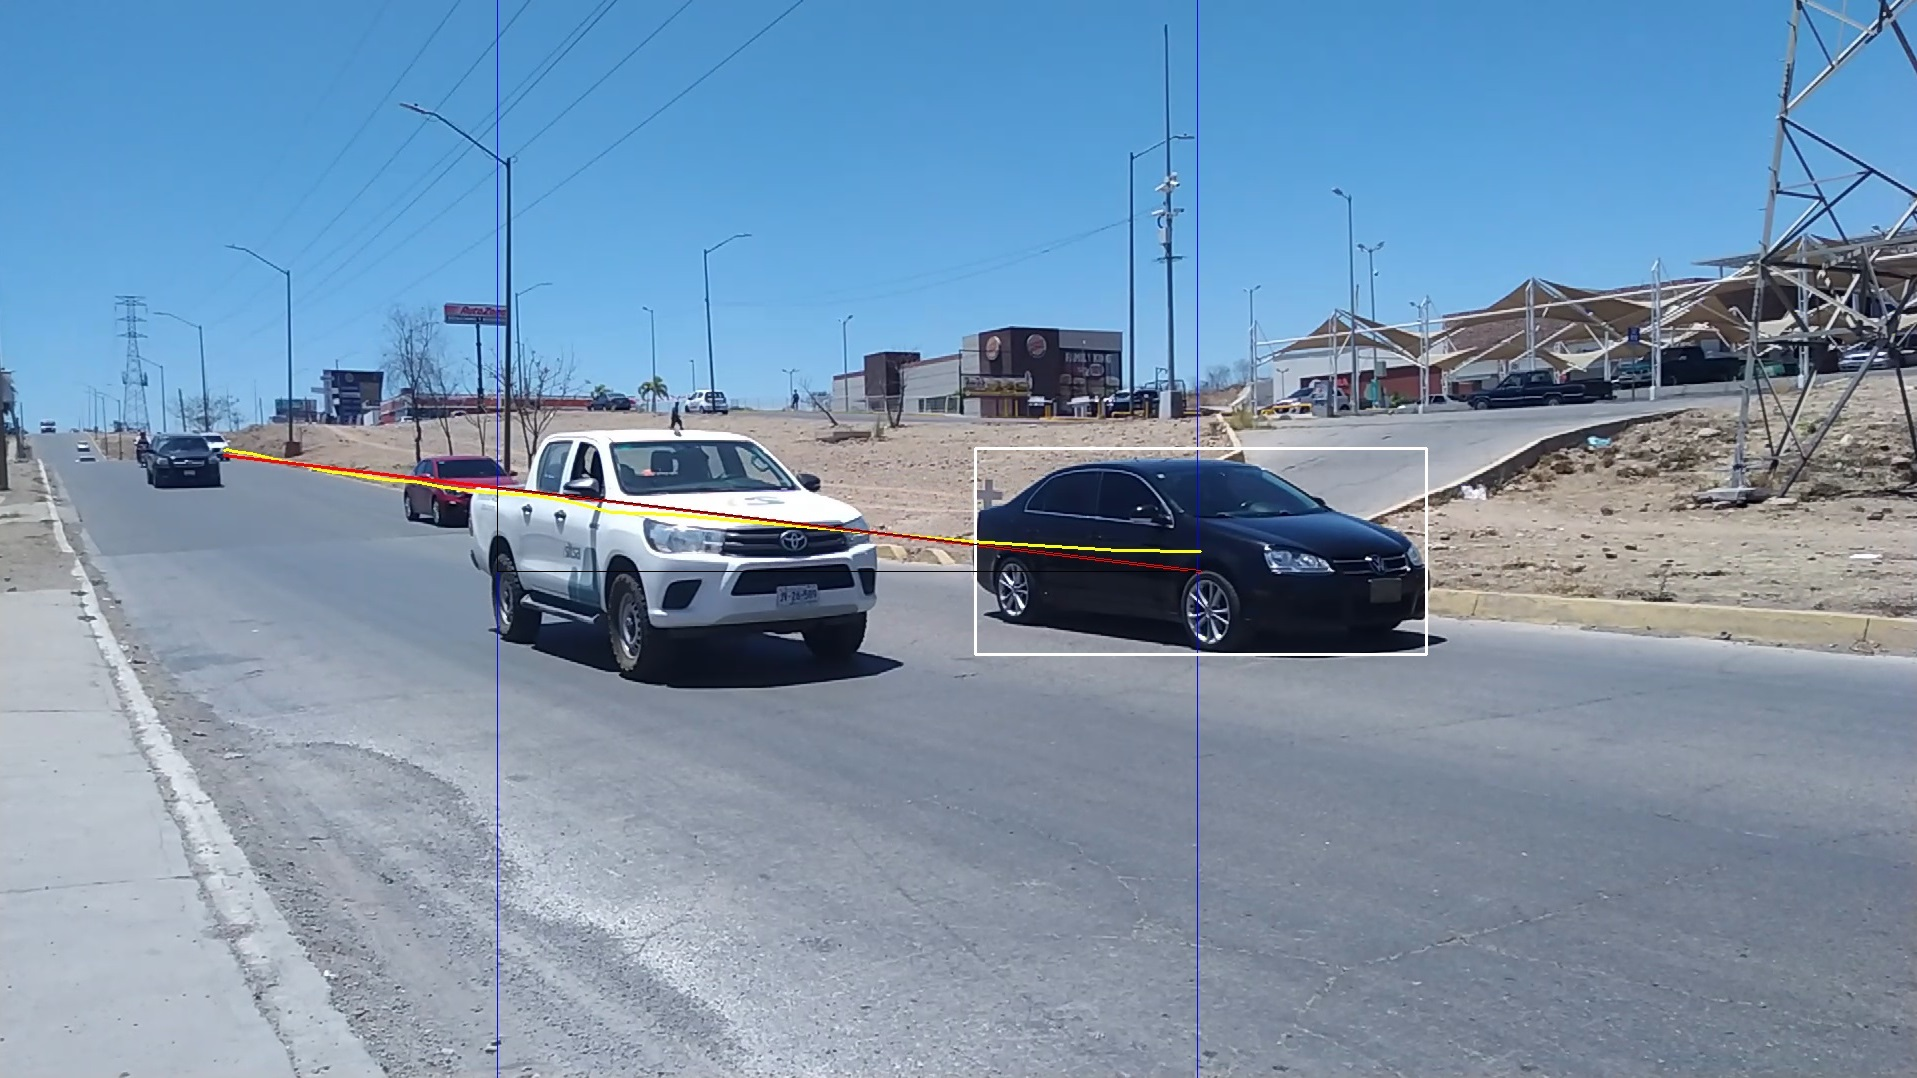
\includegraphics[width=0.8\textwidth]{Metodologia/imgs/Punto_B.jpg}
    \caption{Punto B con vehículo en recuadro blanco.}
    \label{fig:PuntoB}
\end{figure}

La Tabla \ref{tab:CaracteristicasSistema} muestra las características más importante que son extraídas por el sistema y una descripción.

\begin{table}[H]
    \caption{Características obtenidas por el sistema.}
    \label{tab:CaracteristicasSistema}
    \begin{tabular}{|l|l|}
        \hline
        \textbf{Característica} & \multicolumn{1}{c|}{\textbf{Descripción}} \\ \hline
        \textbf{Ángulo Salida} & Ángulo a partir del punto de entrada hasta el punto de salida \\ \hline
        \textbf{Distancia de salida} & Distancia recorrida desde el punto de entrada hasta el punto de salida \\ \hline
        \textbf{Área Entrada} & Área detectada del vehículo en pixeles en el punto de entrada \\ \hline
        \textbf{Área Salida} & Área detectada del vehículo en pixeles en el punto de salida \\ \hline
        \textbf{FPS} & Fotogramas por segundo del video \\ \hline
        \textbf{Tiempo} & Tiempo que le tomo al vehículo para pasar del punto entrada al de salida \\ \hline
        \textbf{Velocidad} & Velocidad detectada por el radar \\ \hline
        \textbf{Carril} & Carril por que pasa el vehículo \\ \hline
        \textbf{Identificador} & Identificador correspondiente a una imagen generada \\ \hline
    \end{tabular}
\end{table}


El sistema además de generar un archivo csv, crea una imagen de salida la cual corresponde a una línea del archivo resultante, esta imagen está formada por dos imágenes una al lado de la otra, la imagen de la izquierda representa el vehículo cuando entra en el punto A y la imagen de la derecha es cuando el vehículo pasa por el punto B. La Figura \ref{fig:Completo} muestra un ejemplo de esta imagen de salida.

\begin{figure}[H]
    \centering
    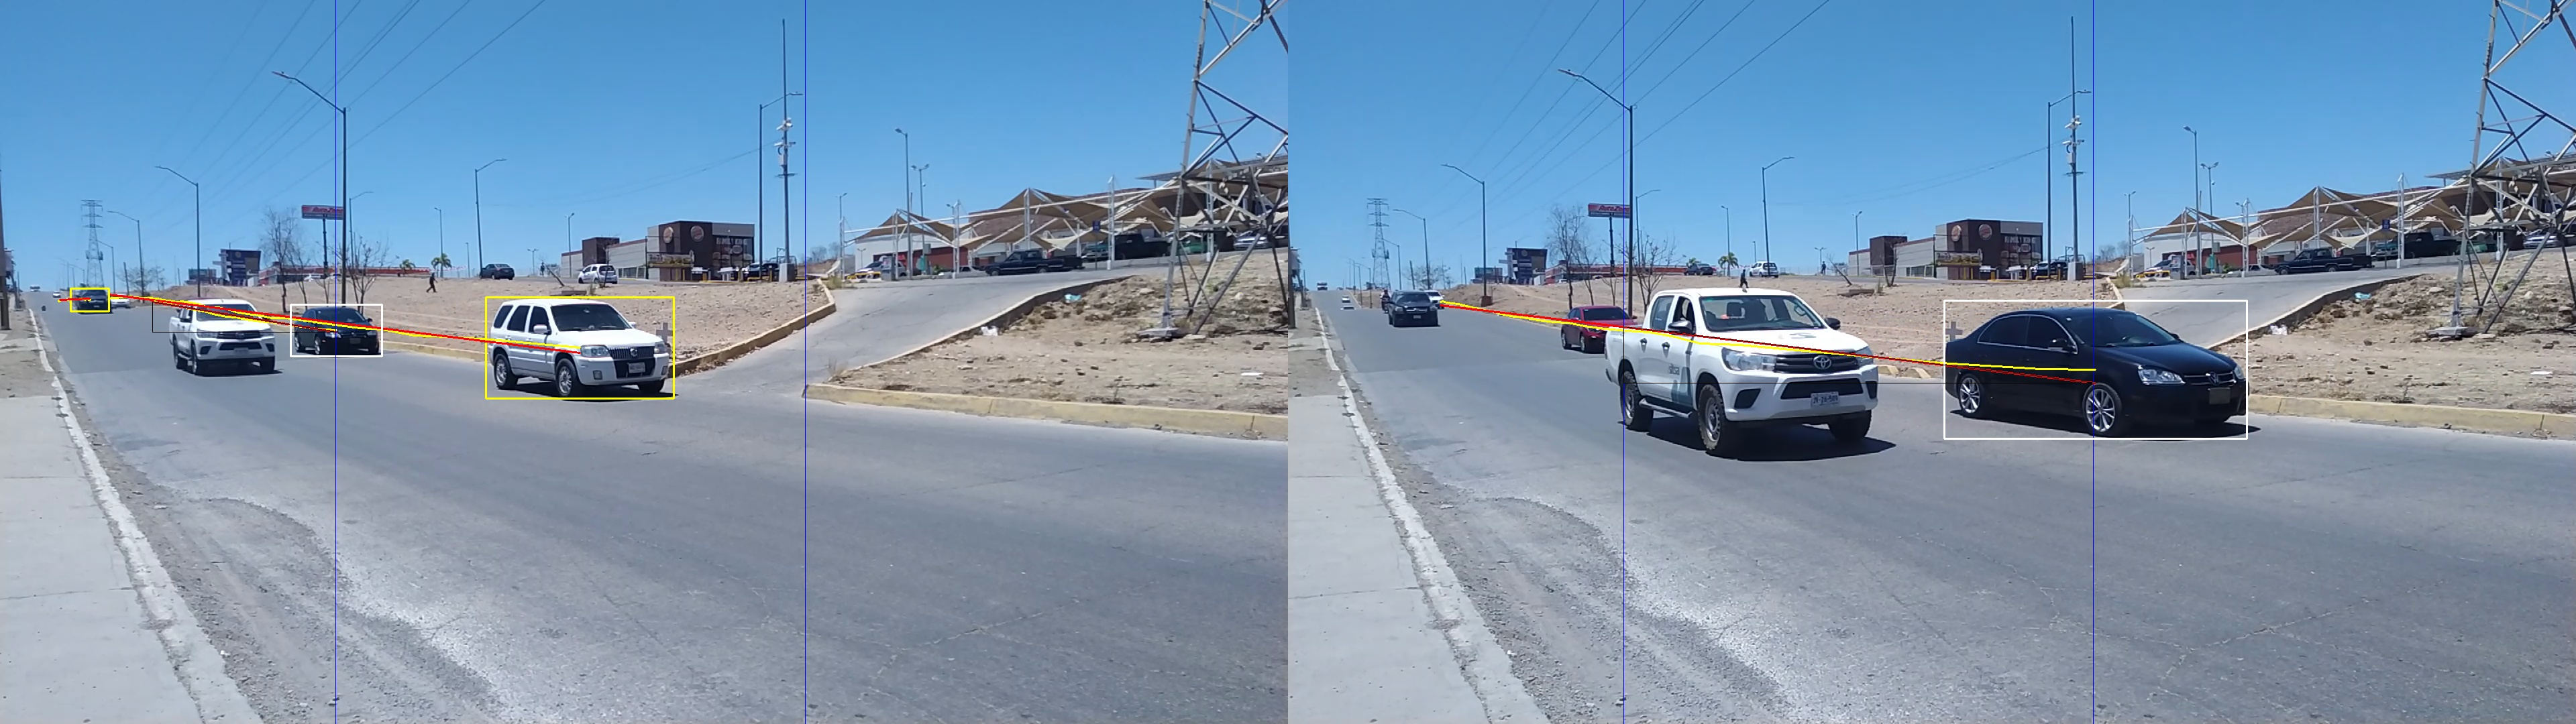
\includegraphics[width=1\textwidth]{Metodologia/imgs/Completo.jpg}
    \caption{Imagen resultado para cada línea de archivo csv.}
    \label{fig:Completo}
\end{figure}

%%%%%%%%%%%%%%%%%%%%%%%%%%%%%%%%%%%%%%%%%%%%%%%%%%%%%%%%%%%%%%%%%%%%%%%%%%%%%%%%
%%%%%%%%%%%%%%%%%%%%%%%%%%%%%%%%%%%%%%%%%%%%%%%%%%%%%%%%%%%%%%%%%%%%%%%%%%%%%%%%
%%%%%%%%%%%%%%%%%%%%%%%%%%%%%%%%%%%%%%%%%%%%%%%%%%%%%%%%%%%%%%%%%%%%%%%%%%%%%%%%
%%%%%%%%%%%%%%%%%%%%%%%%%%%%%%%%%%%%%%%%%%%%%%%%%%%%%%%%%%%%%%%%%%%%%%%%%%%%%%%%
%%%%%%%%%%%%%%%%%%%%%%%%%%%%%%%%%%%%%%%%%%%%%%%%%%%%%%%%%%%%%%%%%%%%%%%%%%%%%%%%

Una vez que el sistema genera las imágenes de salida. El archivo csv resultante valida que el vehículo detectado sea el correcto y que el recuadro blanco que define la detección del vehículo contenga la mayor parte del vehículo.

Para el caso de validar que el vehículo sea el correcto, es necesario ver cada una de las imágenes generadas y leer la descripción en el archivo csv de entrada. En caso de identificar un vehículo que no corresponda, se debe modificar los segundos en el archivo csv de entrada de tal manera que el sistema detecte el vehículo  correcto, esto implica ejecutar el sistema nuevamente para generar los datos de nuevo. 

Existen dos casos en los que el sistema no podrá identificar el vehículo. El primer caso implica que el vehículo sea obstaculizado por otro. Por lo cual, la detección será del vehículo que esta frente al vehículo que se le esta realizando el seguimiento. El segundo caso corresponde cuando al vehículo no se le realizo el seguimiento completo del punto A al B de forma correcta, esto implica que el vehículo no fue detectado en el camino. Para estos dos caso se elimina la línea correspondiente en el archivo de entrada, lo cual también implica ejecutar el sistema nuevamente para generar los datos nuevamente.


Para validar que el área de detección del vehículo sea completa, se realizó una inspección visual de las imágenes generadas. Durante la inspección se identifica
el vehículo cuando entra en el punto A (Figura \ref{fig:ImagenValida01}) el cual debe ser detectado completamente por el recuadro blanco, al mismo tiempo que se identifica el vehículo cuando pasa por el punto B (Figura \ref{fig:ImagenValida02}) el cual también debe ser identificado completamente por el recuadro blanco.


\begin{figure}[H]
    \centering
    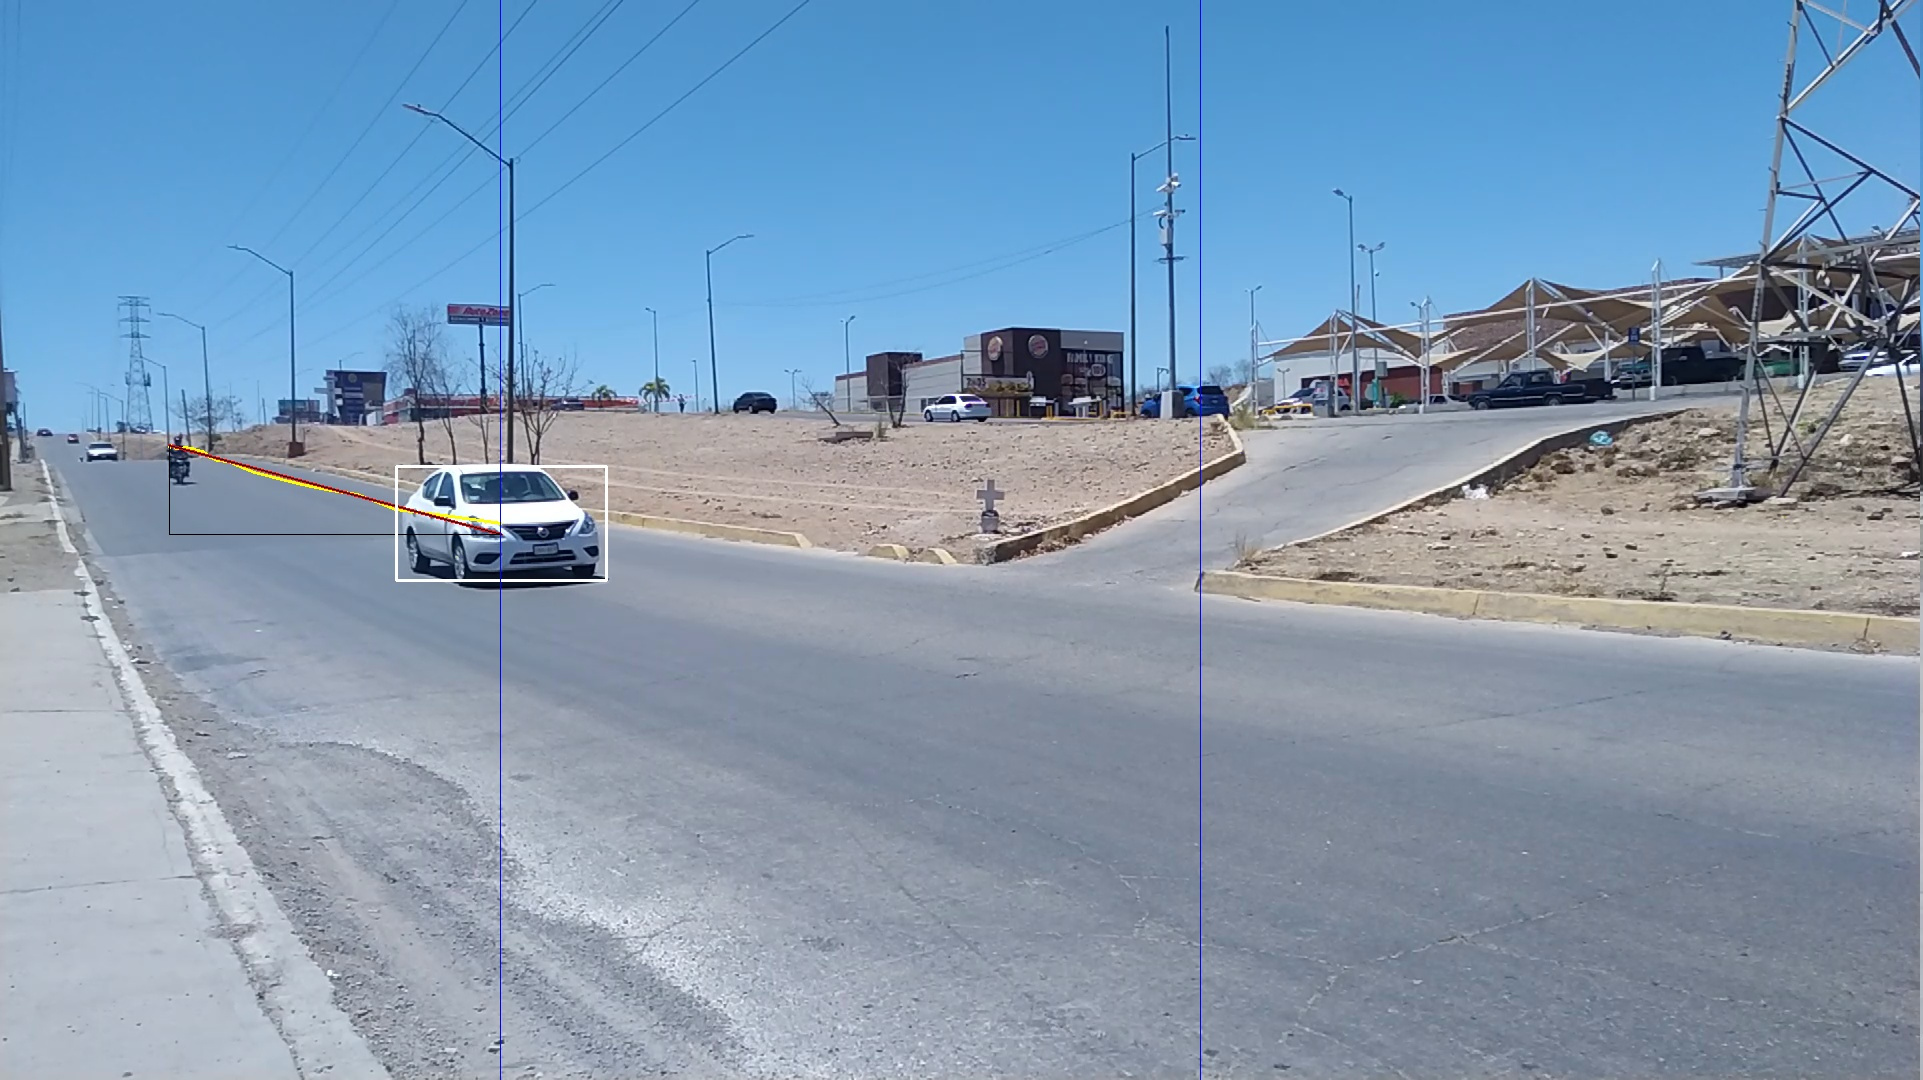
\includegraphics[width=0.8\textwidth]{Metodologia/imgs/Valido_001.jpg}
    \caption{Imagen válida con vehículo entrando representando una línea del archivo csv.}
    \label{fig:ImagenValida01}
\end{figure}

\begin{figure}[H]
    \centering
    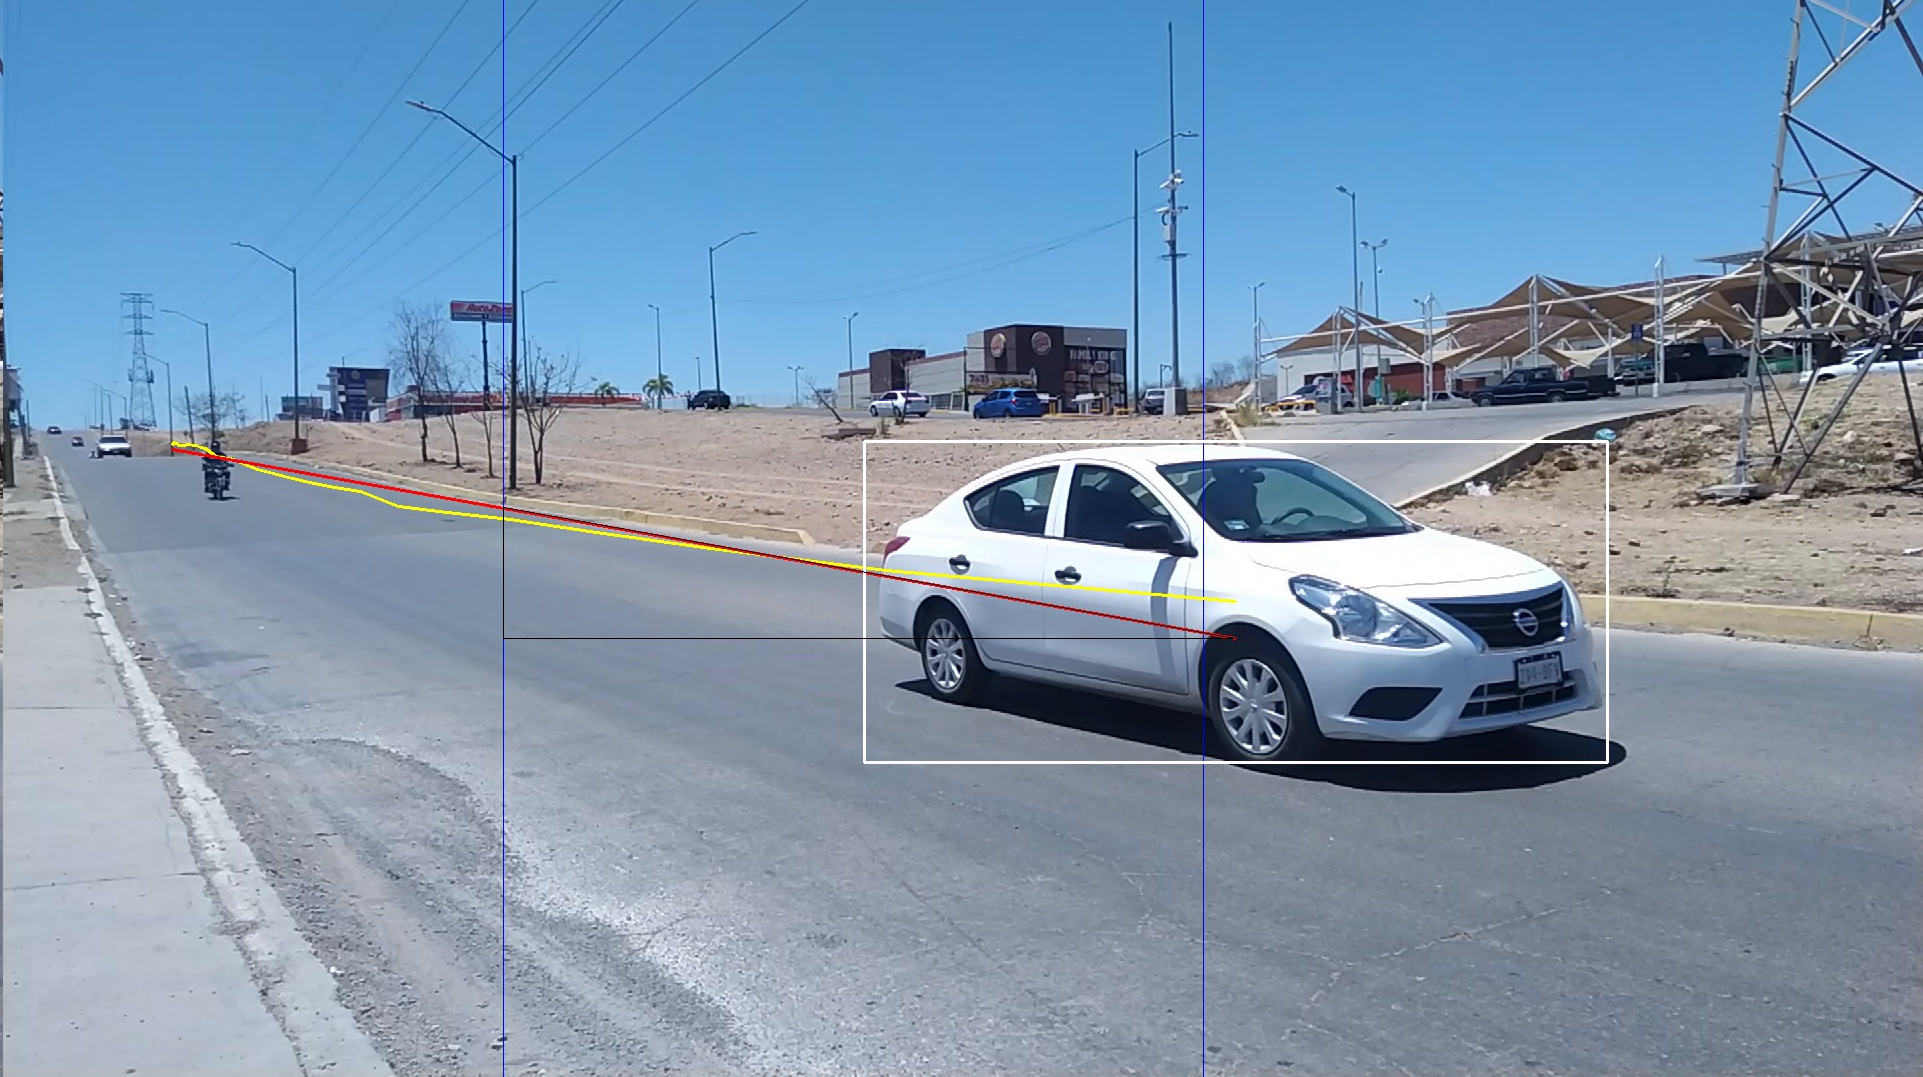
\includegraphics[width=0.8\textwidth]{Metodologia/imgs/Valido_002.jpg}
    \caption{Imagen válida con vehículo saliendo representando una línea del archivo csv.}
    \label{fig:ImagenValida02}
\end{figure}

Por otra parte, hay ocasiones en la cuales el sistema solo detecta parte del vehículo. En este caso la muestra se considera como inválida. Un ejemplo, la Figura \ref{fig:ImagenInvalida_01} muestra el vehículo detectado completamente en el punto A, mientras que cuando el vehículo sale por el punto B es detectado solo una parte (Figura \ref{fig:ImagenInvalida_02}).

\begin{figure}[H]
    \centering
    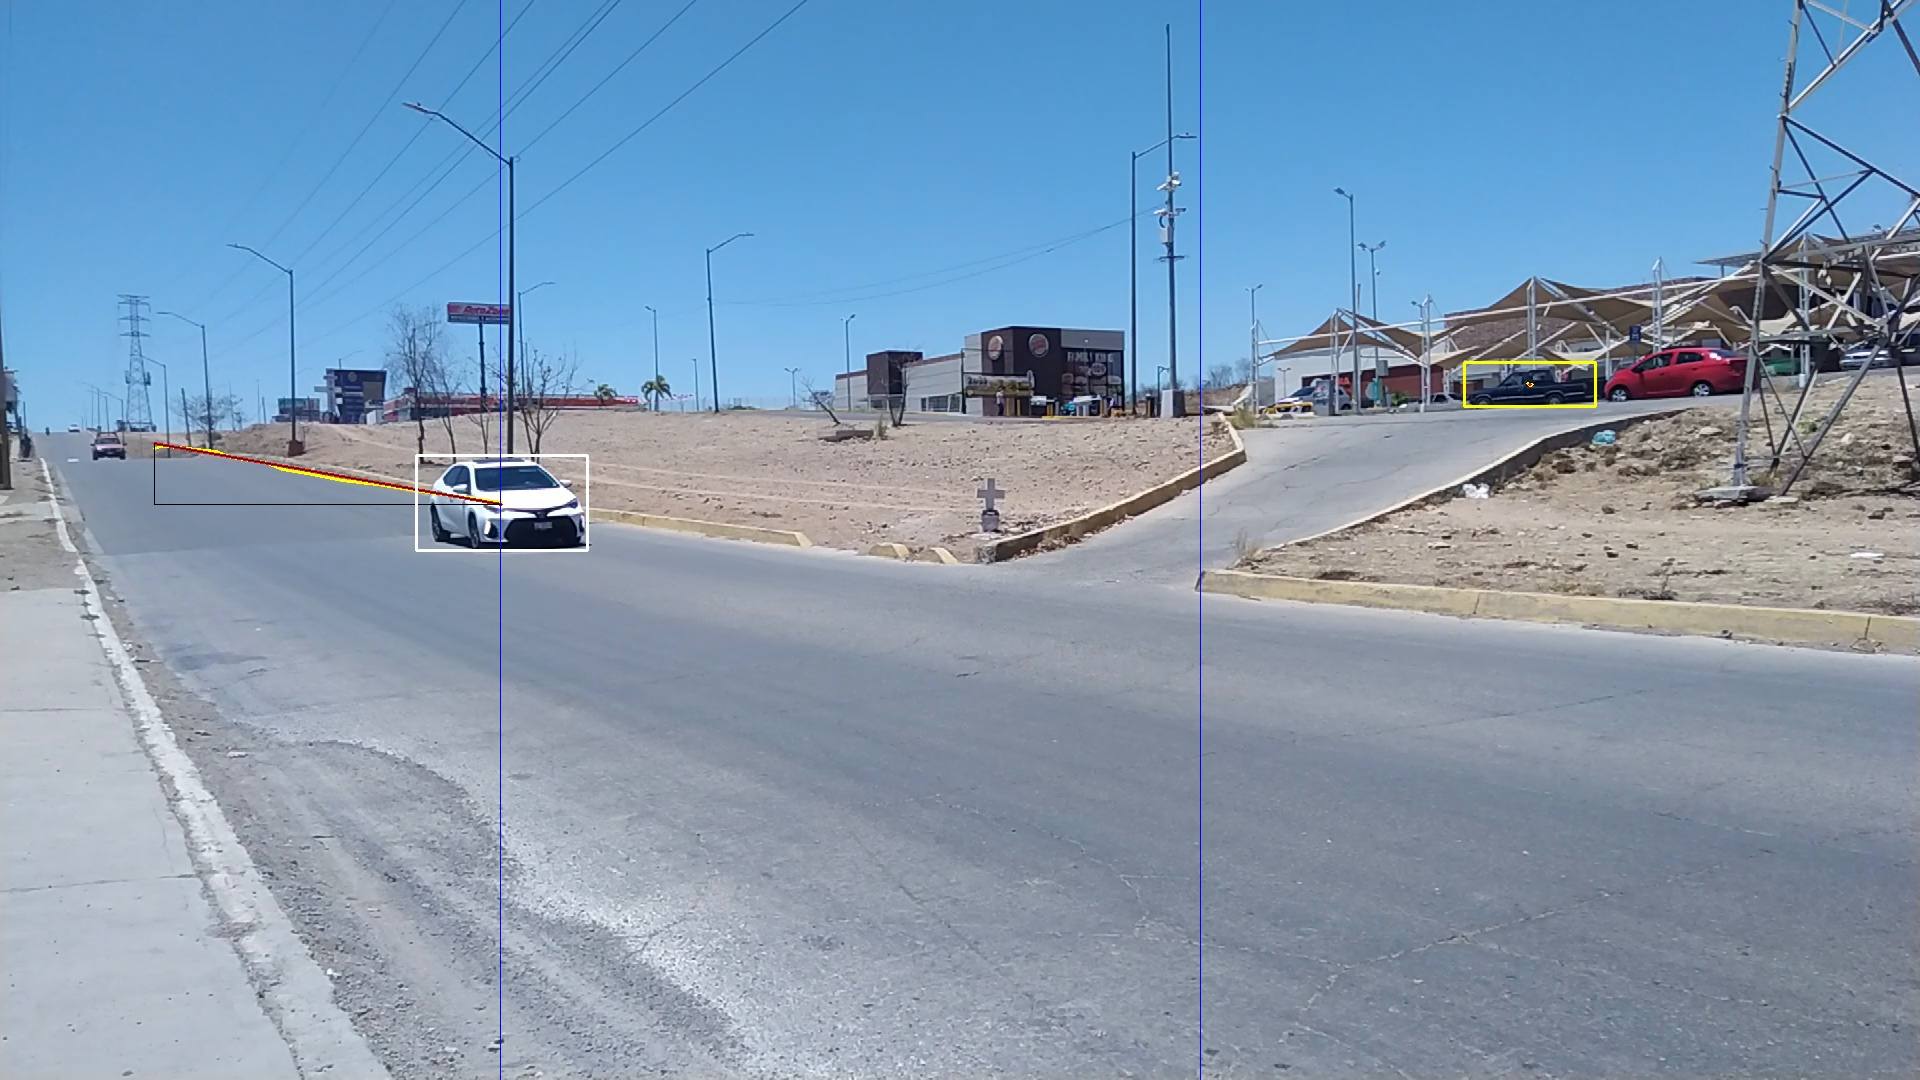
\includegraphics[width=0.8\textwidth]{Metodologia/imgs/Invalido_001.jpg}
    \caption{Imagen inválida (parte izquierda) con vehículo entrando representando una línea del archivo csv.}
    \label{fig:ImagenInvalida_01}
\end{figure}

\begin{figure}[H]
    \centering
    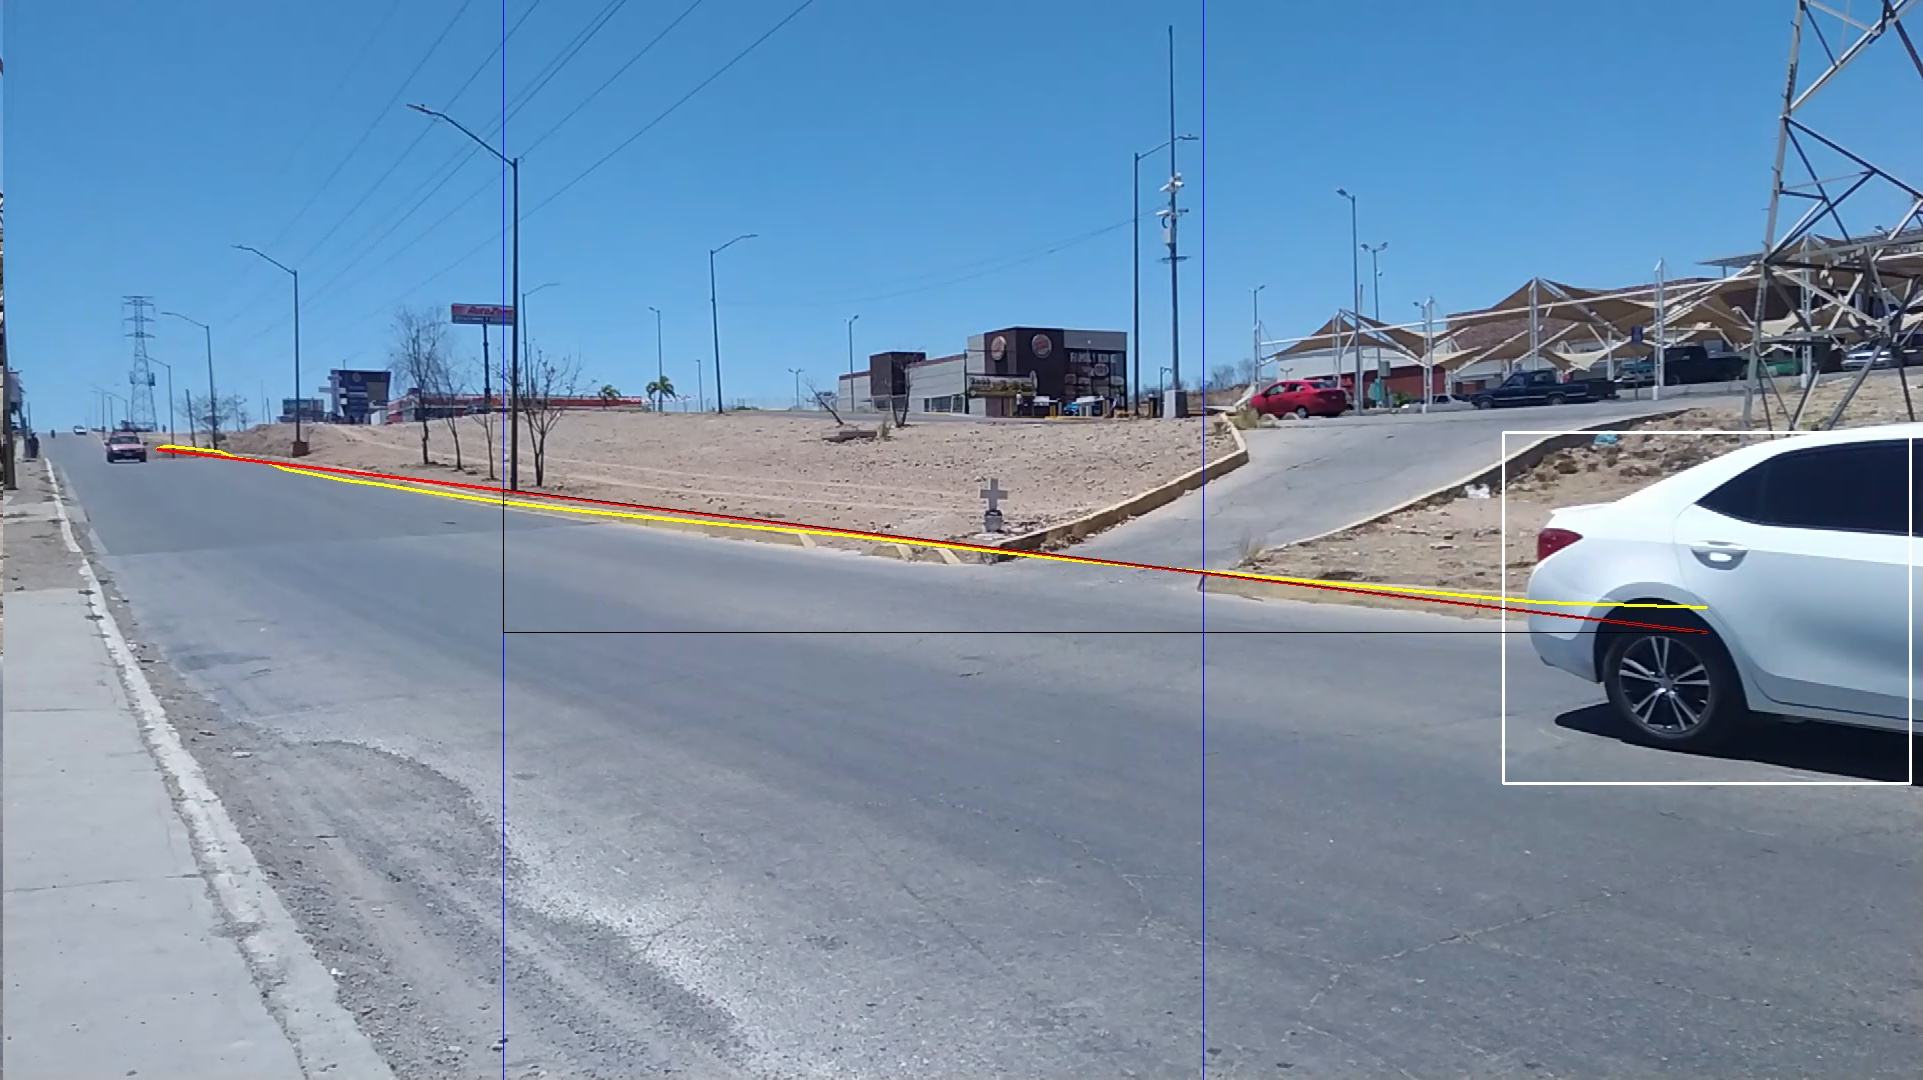
\includegraphics[width=0.8\textwidth]{Metodologia/imgs/Invalido_002.jpg}
    \caption{Imagen inválida (parte derecha) con vehículo saliendo representando una línea del archivo csv.}
    \label{fig:ImagenInvalida_02}
\end{figure}

Una vez que se identifica una imagen inválida se elimina la muestra correspondiente en el archivo csv de salida. Esta muestra se reconoce por el identificador descrito en la Tabla \ref{tab:CaracteristicasSistema}. Para este caso no es necesario volver a ejecutar el sistema.


\subsection{Modelo predictivo}
\label{cap:EstimacionVelocidad}

En esta sección se describe la metodología utilizada para crear un proceso o modelo el cual podamos utilizar para determinar la velocidad de vehículos, se implementaron dos metodologías para esta tarea, el primero utiliza la fórmula física de la velocidad, a partir de esta fórmula se busca un factor de correlación entre la distancia en pixeles recorrida por el vehículo y la distancia real, mientras que el segundo método implementado es el entrenamiento de un modelo de aprendizaje máquina utilizando bibliotecas de Python las cuales nos ayudan a crear un modelo con el cual podemos determinar la velocidad.

\subsubsection{Estimar velocidad basado en factor de correlación}

Para determinar la velocidad utilizando el conjunto de datos generado por el sistema se inicia a partir de lo más sencillo utilizando la fórmula física para el cálculo de la velocidad, Ecuación \ref{eq:Velocidad}.

\begin{equation}
    \label{eq:Velocidad}
    Velocidad = \frac{Distancia}{Tiempo}
\end{equation}

En este caso las muestras fueron tomadas por un Radar que solo nos proporciona la velocidad en Kilómetros o en Millas, así que necesitamos convertir este valor a Metros sobre segundo, utilizando la Ecuación \ref{eq:ConvertMSKH}.

\begin{equation}
    \label{eq:ConvertMSKH}
    \frac{M}{S} = \frac{18}{5} \times \frac{K}{H}
\end{equation}

A partir de la formula física para el cálculo de la velocidad y la conversión de la velocidad en metros por segundo en lugar de kilómetros por hora, podemos definir el proceso para crear el modelo en el diagrama de flujo que se muestra en la Figura \ref{fig:CrearModeloCustom}.

\begin{figure}[H]
    \centering
    \begin{tikzpicture}
        \node(a)[circle, draw=black, minimum size=1.5cm]
            {Inicio};

        \node(b)[rectangle, draw=black, minimum width=5cm, minimum height=1.7cm]
            [right=of a]
            [text width=5cm, align=center]
            {Calcular distancia estimada};
        \node(c)[rectangle, draw=black, minimum width=5cm, minimum height=1.7cm]
            [right=of b]
            [text width=5cm, align=center]
            {Encontrar factor de correlación};
        \node(d)[rectangle, draw=black, minimum width=5cm, minimum height=1.7cm]
            [below=of c]
            [text width=5cm, align=center]
            {Promediar factor de correlación};
        \node(e)[rectangle, draw=black, minimum width=5cm, minimum height=1.7cm]
            [left=of d]
            [text width=5cm, align=center]
            {Integrar factor de correlación con formula de velocidad};

        \node(f)[circle, draw=black, minimum size=1.5cm]
            [left=of e]
            {Fin};

        \draw[->] (a) -- (b);
        \draw[->] (b) -- (c);

        \draw[->] (c) -- (d);
        \draw[->] (d) -- (e);
        \draw[->] (e) -- (f);


    \end{tikzpicture}

    \caption{Diagrama de flujo para la creación de modelo con la formula física de la velocidad.}
    \label{fig:CrearModeloCustom}
\end{figure}

La Tabla \ref{tab:CaracteristicasSistema} muestra que los tres parámetros necesarios para estimar la velocidad, sin embargo, el valor de la distancia está en pixeles, por lo que es necesario convertir el valor a una distancia estimada, este valor es convertido con la Ecuación \ref{eq:Velocidad} despejando la distancia, con esto se obtiene la  Ecuación \ref{eq:DistanciaEstimada}.

\begin{equation}
    \label{eq:DistanciaEstimada}
    Distancia\:Estimada = Tiempo \times Velocidad
\end{equation}

Una vez que se tiene la distancia estimada, debemos encontrar la correlación entre esta y la distancia en pixeles, con lo cual tenemos la siguiente Ecuación \ref{eq:EcuacionB}.

\begin{equation}
    \label{eq:EcuacionB}
    B = \frac{Distancia \: Estimada}{Distancia \: Pixeles}
\end{equation}

A este valor lo llamamos simplemente B, el valor de B es utilizado para calcular una velocidad estimada con respecto a la distancia y el tiempo, lo cual quedaría como muestra la Ecuación \ref{eq:VelocidadB}.

\begin{equation}
    \label{eq:VelocidadB}
    Velocidad = \frac{Distancia \: Pixeles}{Tiempo} \times B
\end{equation}

Sin embargo, esta fórmula solo servirá para un dato en específico generado por el sistema por lo cual debemos encontrar un valor de B que modele la gran mayoría de nuestras muestras o tener un error lo más bajo posible, para esto se calcula el valor de B para todas las muestras y se calcula el promedio de B, Ecuación \ref{eq:PromedioB}.

\begin{equation}
    \label{eq:PromedioB}
    \overline{B} = \frac{\sum B}{n}
\end{equation}

Una vez se tiene B promedio se puede sustituir por B en la Ecuación \ref{eq:VelocidadB} lo cual quedaría como muestra la Ecuación \ref{eq:VelocidadBPromedio}.

\begin{equation}
    \label{eq:VelocidadBPromedio}
    Velocidad = \frac{Distancia \: Pixeles}{Tiempo} \times \overline{B}
\end{equation}



\subsubsection{Estimar velocidad Scikit y Tensor Flow}

El proceso de creación del modelo de Scikit y Tensor Flow son el mismo, este se describe en el diagrama de flujo de la Figura \label{ref:ModeloScikitTensorFlow}.

\begin{figure}[H]
    \centering
    \begin{tikzpicture}[node distance=5mm]

        \node(a)[circle, draw=black, minimum size=1cm]
            {Inicio};

        \node(b)[rectangle, draw=black, minimum width=3cm, minimum height=1.2cm]
            [right=of a]
            [text width=3cm, align=center]
            {Separar conjunto de datos};
        \node(c)[rectangle, draw=black, minimum width=3cm, minimum height=1.2cm]
            [right=of b]
            [text width=3cm, align=center]
            {Entrenar modelo};
        \node(d)[rectangle, draw=black, minimum width=3cm, minimum height=1.2cm]
            [right=of c]
            [text width=3cm, align=center]
            {Validar modelo};


        \node(e)[circle, draw=black, minimum size=1cm]
            [right=of d]
            {Fin};

        \draw[->] (a) -- (b);
        \draw[->] (b) -- (c);
        \draw[->] (c) -- (d);
        \draw[->] (d) -- (e);
    \end{tikzpicture}
    \caption{Diagrama de flujo para estimar velocidad utilizando inteligencia artificial.}
    \label{fig:ModeloScikitTensorFlow}
\end{figure}


El proceso para entrenar un modelo tanto en Scikit como Tensor Flow es el proceso más común utilizado. El primer paso es separar el conjunto de datos en un conjunto de entrenamiento y otro de validación normalmente esto se realiza en un porcentaje de 70\% - 30\%. Una vez separado el conjunto de datos se procede al entrenamiento utilizando la herramienta elegida, hasta que se tiene una precisión tan buena como se requiera. Por último, se utiliza el modelo con el conjunto de validación para garantizar que los resultados obtenidos sean tan buenos como en el conjunto de entrenamiento.


\subsection{Obtención de la velocidad}

Utilizando el conjunto de datos creado por el sistema para generar el modelo que se propone en la Sección \ref{cap:EstimacionVelocidad} podemos determinar la velocidad simplemente adquiriendo los datos de la distancia en pixeles y el tiempo más nuestra B promedio, con esto es solo cuestión de sustituir los valores en la Ecuación \ref{eq:VelocidadBPromedio}.

Por ejemplo, calculamos nuestra B promedio la cual es igual a 0.0162, el sistema obtiene la distancia en pixeles y el tiempo que le tomo si vehículo pasar del punto A al punto B, los cuales son igual a 962 y 0.933 respectivamente, ahora solo es cuestión de sustituir estos valores para conseguir la velocidad estimada.

\begin{equation}
    \label{eq:EjemploImplementacion}
    Velocidad = \frac{962 }{0.933} \times 0.0162 = 16.703 \: m/s
\end{equation}


No obstante, esta estimación está en M/S, entonces debemos convertirlo a K/H de la siguiente manera.

\begin{equation}
    \label{eq:EjmploKH}
     16.703\times \frac{18}{5} = 60.13 \: k/h
\end{equation}

Este es el resultado de estimar la velocidad de un vehículo utilizando el método propuesto, por otro lado, este es un método simple el cual nos ayudó como punto de referencia para futuros experimentos, por ejemplo, usando bibliotecas como Scikit para utilizar modelos ya existentes en esta biblioteca o Tensor Flow para crear una red neuronal con las características que mejor se adecuen a este caso.


%%%%%%%%%%%%%%%%%%%%%%%%%%%%%%%%%%%%%%%%%%%%%%%%%%%%%
%                   APÉNDICES                       %
%%%%%%%%%%%%%%%%%%%%%%%%%%%%%%%%%%%%%%%%%%%%%%%%%%%%%
%\appendix
%% this file is called up by thesis.tex
% content in this file will be fed into the main document
\chapter{Código/Manuales/Publicaciones}
% top level followed by section, subsection

\section{Apéndice}

Apéndice
               % Colocar los circuitos, manuales, código fuente, pruebas de teoremas, etc.

%%%%%%%%%%%%%%%%%%%%%%%%%%%%%%%%%%%%%%%%%%%%%%%%%%%%%
%                   REFERENCIAS                     %
%%%%%%%%%%%%%%%%%%%%%%%%%%%%%%%%%%%%%%%%%%%%%%%%%%%%%

\phantomsection
\addcontentsline{toc}{chapter}{Bibliograf\'ia}
% existen varios estilos de bilbiografía, pueden cambiarlos a placer


% \bibliographystyle{apalike} % otros estilos pueden ser abbrv, acm, alpha, apalike, ieeetr, plain, siam, unsrt

%El formato trae otros estilos, o pueden agregar uno que les guste:
%\bibliographystyle{Latex/Classes/PhDbiblio-case} % title forced lower case
%\bibliographystyle{Latex/Classes/PhDbiblio-bold} % title as in bibtex but bold
%\bibliographystyle{Latex/Classes/PhDbiblio-url} % bold + www link if provided
%\bibliographystyle{Latex/Classes/jmb} % calls style file jmb.bst

\begingroup
\setstretch{2.0}
\printbibliography
\endgroup
% \begin{spacing}{1.5}
% \printbibliography
% \end{spacing}
% \bibliography{Bibliografia/referencias}             % Archivo .bib




\end{document}
